\documentclass[11pt]{article}

%\geometry{showframe}% for debugging purposes -- displays the margins

\newcommand{\E}{\mbox{E}}
\newcommand{\MSE}{\mbox{MSE}}
\newcommand{\var}{\mbox{var}}
\newcommand{\bx}{\mathbf{x}}

%% ys
\usepackage[shortlabels]{enumitem}
\usepackage{geometry}
\usepackage{bm}
\usepackage{amssymb}
\usepackage{algorithm}
\usepackage{algpseudocode}
\usepackage{xcolor}
\usepackage{listings}
\geometry{a4paper,scale=0.75}
\newcommand{\jie}{$\star$ }
\renewcommand{\bx}{\bm{x}}
\newcommand{\iid}{\overset{\text{iid}}{\sim}}
\newcommand{\half}{\frac{1}{2}}
\newcommand{\ynote}[1]{\color{red} #1 \color{black}}

\usepackage{graphicx}
\usepackage{fancyvrb}
\usepackage{listings}
\usepackage{bm}
\usepackage{xcolor}
\usepackage{caption}
\usepackage{subcaption}
\usepackage{graphicx}

\xdefinecolor{gray}{rgb}{0.4,0.4,0.4}
\xdefinecolor{blue}{RGB}{58,95,205}% R's royalblue3; #3A5FCD

\lstset{% setup listings
	language=R,% set programming language
	basicstyle=\ttfamily\small,% basic font style
	keywordstyle=\color{blue},% keyword style
        commentstyle=\color{gray},% comment style
	numbers=left,% display line numbers on the left side
	numberstyle=\scriptsize,% use small line numbers
	numbersep=10pt,% space between line numbers and code
	tabsize=3,% sizes of tabs
	showstringspaces=false,% do not replace spaces in strings by a certain character
	captionpos=b,% positioning of the caption below
        breaklines=true,% automatic line breaking
        escapeinside={(*}{*)},% escaping to LaTeX
        fancyvrb=true,% verbatim code is typset by listings
        extendedchars=false,% prohibit extended chars (chars of codes 128--255)
        %literate={"}{{\texttt{"}}}1{<-}{{$\bm\leftarrow$}}1{<<-}{{$\bm\twoheadleftarrow$}}1
        %{~}{{$\bm\sim$}}1{<=}{{$\bm\le$}}1{>=}{{$\bm\ge$}}1{!=}{{$\bm\neq$}}1{^}{{$^{\bm\wedge}$}}1,% item to replace, text, length of chars
        alsoletter={.<-},% becomes a letter
        alsoother={\$},% becomes other
        otherkeywords={!=, ~, \$, \&, \%/\%, \%*\%, \%\%, <-, <<-, /},% other keywords
        deletekeywords={c}% remove keywords
}
%% ys

\usepackage{amsmath}
%\usepackage[garamond]{mathdesign}
\usepackage{url}

% Set up the images/graphics package
\usepackage{graphicx}
\setkeys{Gin}{width=\linewidth,totalheight=\textheight,keepaspectratio}
\graphicspath{{graphics/}}

\title{Exercises 4 $\cdot$ SSC 383D \\ Exercises 5: Hierarchical Linear Models}
%\author[ ]{ }
\date{}  % if the \date{} command is left out, the current date will be used

% The following package makes prettier tables.  We're all about the bling!
\usepackage{booktabs}

% The units package provides nice, non-stacked fractions and better spacing
% for units.
\usepackage{units}

% The fancyvrb package lets us customize the formatting of verbatim
% environments.  We use a slightly smaller font.
\usepackage{fancyvrb}
\fvset{fontsize=\normalsize}

% Small sections of multiple columns
\usepackage{multicol}

% Provides paragraphs of dummy text
\usepackage{lipsum}

% These commands are used to pretty-print LaTeX commands
\newcommand{\doccmd}[1]{\texttt{\textbackslash#1}}% command name -- adds backslash automatically
\newcommand{\docopt}[1]{\ensuremath{\langle}\textrm{\textit{#1}}\ensuremath{\rangle}}% optional command argument
\newcommand{\docarg}[1]{\textrm{\textit{#1}}}% (required) command argument
\newenvironment{docspec}{\begin{quote}\noindent}{\end{quote}}% command specification environment
\newcommand{\docenv}[1]{\textsf{#1}}% environment name
\newcommand{\docpkg}[1]{\texttt{#1}}% package name
\newcommand{\doccls}[1]{\texttt{#1}}% document class name
\newcommand{\docclsopt}[1]{\texttt{#1}}% document class option name

\newcommand{\N}{\mbox{N}}
\newcommand{\thetahat}{\hat{\theta}}
\newcommand{\sigmahat}{\hat{\sigma}}
\newcommand{\betahat}{\hat{\beta}}


\begin{document}

\maketitle% this prints the handout title, author, and date


\section{Price elasticity of demand}

The data in ``cheese.csv'' are about sales volume, price, and advertisting display activity for packages of Borden sliced ``cheese.'' The data are taken from Rossi, Allenby, and McCulloch's textbook on \textit{Bayesian Statistics and Marketing.} For each of 88 stores (store) in different US cities, we have repeated observations of the weekly sales volume (vol, in terms of packages sold), unit price (price), and whether the product was advertised with an in-store display during that week (disp = 1 for display).

Your goal is to estimate, on a store-by-store basis, the effect of display ads on the demand curve for cheese.  A standard form of a demand curve in economics is of the form $Q = \alpha P^\beta$, where $Q$ is quantity demanded (i.e.~sales volume), $P$ is price, and $\alpha$ and $\beta$ are parameters to be estimated.  You'll notice that this is linear on a log-log scale,
$$
\log Q = \log \alpha + \beta \log P \,
$$
which you should feel free to assume here.  Economists would refer to $\beta$ as the price elasticity of demand (PED).  Notice that on a log-log scale, the errors enter multiplicatively.

There are several things for you to consider in analyzing this data set.
\begin{itemize}
\item The demand curve might shift (different $\alpha$) and also change shape (different $\beta$) depending on whether there is a display ad or not in the store.
\item Different stores will have very different typical volumes, and your model should account for this.
\item Do different stores have different PEDs?  If so, do you really want to estimate a separate, unrelated $\beta$ for each store?
\item If there is an effect on the demand curve due to showing a display ad, does this effect differ store by store, or does it look relatively stable across stores?
\item Once you build the best model you can using the log-log specification, do see you any evidence of major model mis-fit?
\end{itemize}
Propose an appropriate hierarchical model that allows you to address these issues, and use Gibbs sampling to fit your model.

\bigskip \jie
Denote we have data for $i = 1, \dots, n$ stores and for each store we have observations $j= 1, \dots, N_i$. The quantity demand is denoted as $Q_{i,j}$ and the price is $P_{i.j}$, and $disp_{i,j}$ is the indicator that product is displayed or not. I use the model as follows,
$$\log Q_{i,j} = \beta_{0,i} + \beta_{1,i} \log P_{i,j} + \beta_{2,i} 1(disp_{i,j} = 1) + \beta_{3,i} \log P_{i,j} \cdot 1(disp_{i,j} = 1).$$
This can be rewritten as a linear regression,
$$y_{ij} = x_{ij}^T \beta_i + \epsilon_{ij},$$
where $y_{ij} = \log Q_{i,j}$, $x_{ij} = (1, \log P_{i,j}, 1(disp_{i,j} = 1), \log P_{i,j} \cdot 1(disp_{i,j} = 1) )^T$, and $\beta_i = (\beta_{0,i}, \dots, \beta_{3,i})^T$.
I propose a hierarchical model as follows,
\begin{align*}
    y_{ij} \mid \beta_i, \sigma_i^2 &\sim N(x_{ij}^T \beta_i, \sigma_i^2) \\
    \beta_i \mid \beta, \Sigma &\sim N(\beta, \Sigma = diag(s_1^2, \dots, s_4^2)) \\
    \sigma^2_i &\propto \text{Inv-Ga}(\frac{a}2, \frac{b}2) \\
    a &\sim U(1, 10) \\
    b &\sim U(1, 10) \\
    \beta & \propto 1  \\
    s_j^2 &\sim \text{Inv-Ga}(\frac{a_0}2, \frac{b_0}2) =  \text{Inv-Ga}(\frac{1}2, \frac{1}2) \;\;\;\; j=1,\dots, 4
\end{align*}
Denote $X_i = \begin{bmatrix}
x_{i1}^T \\
\vdots \\
x_{iN_i}^T
\end{bmatrix}$, then the sampling model can also be written as
$$Y_i \mid \beta_i, \sigma_i^2 \sim N_{N_i} (X_i \beta_i , \sigma^2_i I).$$
We can use the Gibbs sampler to obtain posterior samples based on the full conditionals as follows.

The joint posterior:
\begin{align*}
    p(Y_{1:n}, \beta_{1:n}, \beta, \Sigma, \sigma_{1:n}^2) &\propto \prod_{i=1}^n \{ (\sigma_i^2)^{-\frac{N_i}2} \exp \{ - \frac{1}{2\sigma_i^2} (Y_i - X_i \beta_i)^T(Y_i - X_i\beta_i)\}  \\& \;\;\;\; \cdot |\Sigma|^{-\frac{1}2} \exp \{ -\frac{1}2 (\beta_i - \beta)^T \Sigma^{-1} (\beta_i - \beta) \} \cdot (\sigma^2_i)^{-\frac{a}2 - 1} \exp[-\frac{b}{2\sigma^2_i}] \} \\
    &\;\;\;\; \cdot \prod_{j=1}^4 (s_j^2)^{-\frac{1}2 - 1} \exp[-\frac{1}{2s_j^2}] 1(a\in (1,10)) 1(b\in (1,10))
\end{align*}

The full conditionals:
$$p(\beta_i \mid -) = N(\tilde{\mu}_i, \tilde{\Sigma}_i),$$
where $$\tilde{\Sigma}_i = \left( \frac{X_i^TX_i}{\sigma_i^2} + \Sigma^{-1} \right)^{-1} \text{ and } \tilde{\mu}_i = \tilde{\Sigma}_i \left( \frac{X_i^TY_i}{\sigma_i^2} + \Sigma^{-1}\beta \right).$$
$$p(\beta \mid - ) = N(\bar{\beta}, \frac{1}n \Sigma),$$
where $$\bar{\beta} = \frac{1}n \sum_{i=1}^n \beta_i.$$
$$p(\sigma_i^2 \mid -) = \text{Inv-Ga}(\frac{a}2 + \frac{N_i}2, \frac{b}2 + \frac{1}2(Y_i - X_i\beta_i)^T(Y_i - X_i\beta_i)).$$
$$p(s_j^2 \mid -) = \text{Inv-Ga}(\frac{1}2 + \frac{n}2, \frac{1}2 + \frac{1}2\sum_{i=1}^n (\beta_{ij}-\beta_j)^2).$$
$$p(a \mid -) \propto \prod_{i=1}^n (\sigma^2_i)^{-\frac{a}2 -1} 1(a \in (0.5,10)).$$
$$p(b \mid -) \propto \exp[- \sum_{i=1}^n \frac{b}{2\sigma_i^2}] 1(b \in (0.5,10)).$$

After implementing the MCMC, I got the posterior mean estimates of the parameters, and here the $\beta_i$ for each stores are shown in Figure \ref{fig:hist_betai}.
\begin{figure}[h]
    \centering
    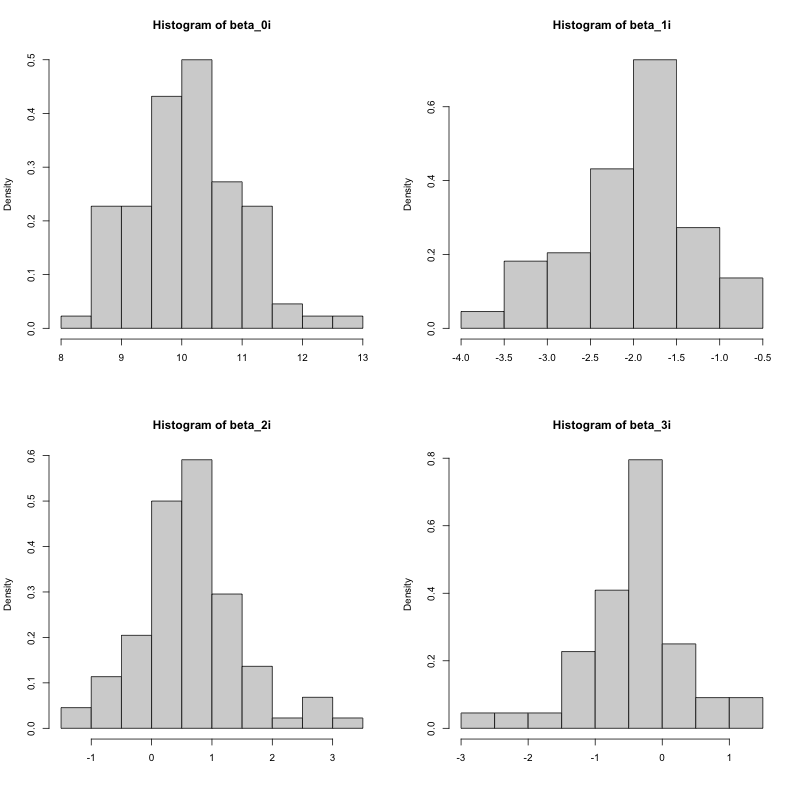
\includegraphics[width=0.8\textwidth]{Ex5/figures/hist_betai.png}
    \caption{Histogram of the posterior mean estimates of the $beta_i$ over the stores.}
    \label{fig:hist_betai}
\end{figure}
\begin{figure}[h]
    \centering
    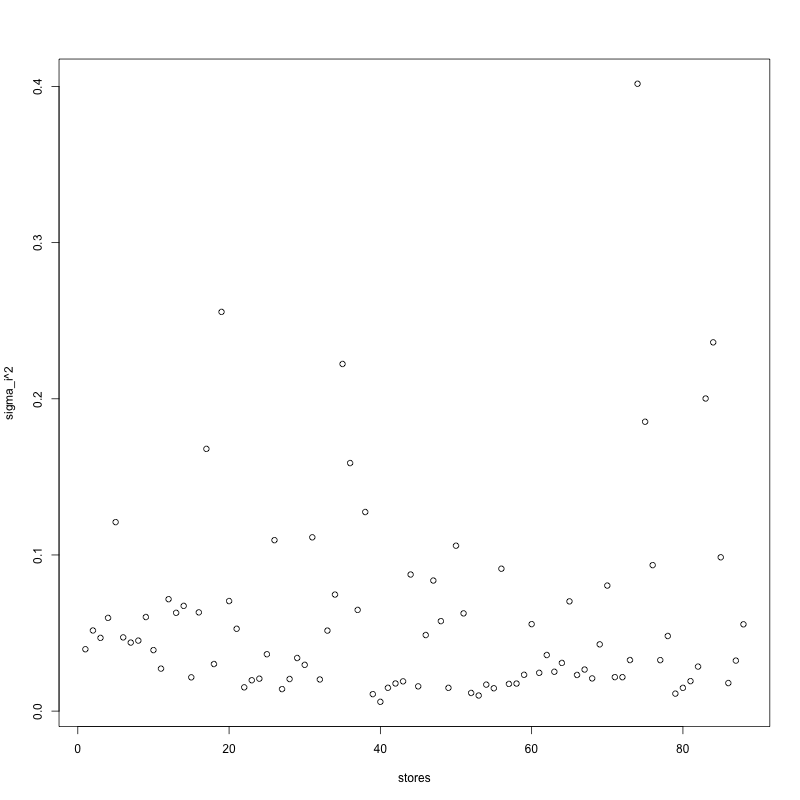
\includegraphics[width=0.6\textwidth]{Ex5/figures/sig.png}
    \caption{Scatter plot of $\sigma_i^2$.}
    \label{fig:hist_betai}
\end{figure}
\begin{figure}[h]
    \centering
    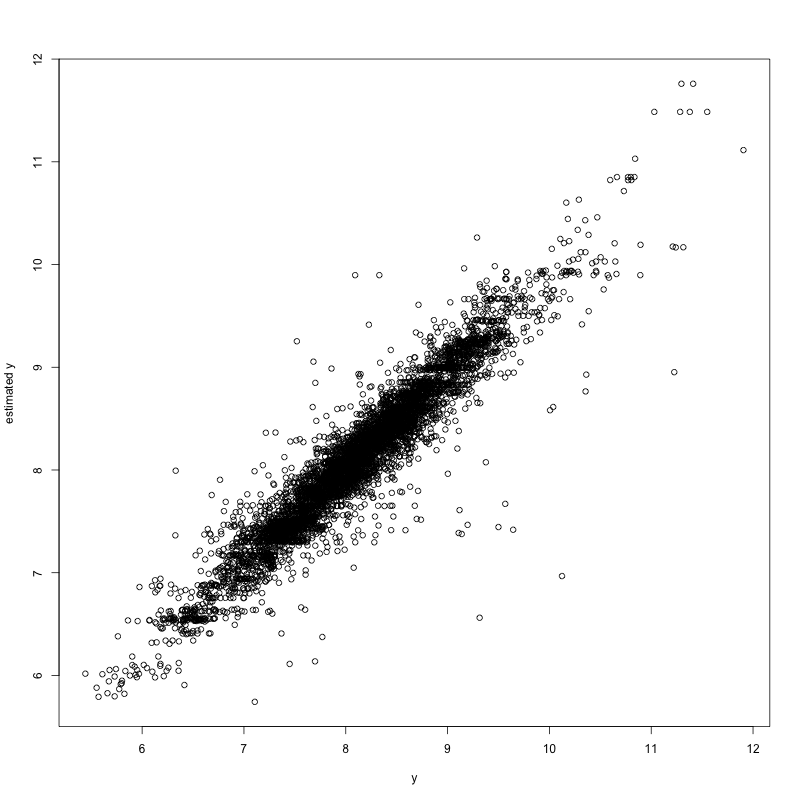
\includegraphics[width=0.6\textwidth]{Ex5/figures/esty.png}
    \caption{True y against estimated y.}
    \label{fig:hist_betai}
\end{figure}
\begin{figure}
    \centering
    \begin{subfigure}[t]{0.45\textwidth}
        \centering
        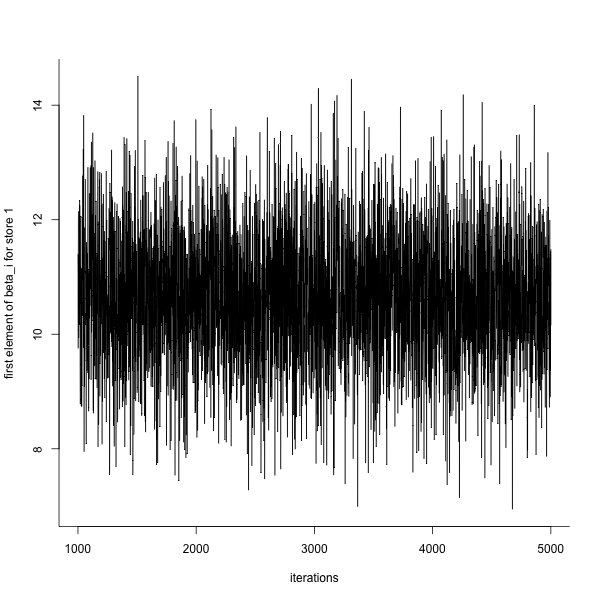
\includegraphics[width=\linewidth]{Ex5/figures/tra_betai.png} 
        %\caption{Generic} \label{fig:timing1}
    \end{subfigure}
    \hfill
    \begin{subfigure}[t]{0.45\textwidth}
        \centering
        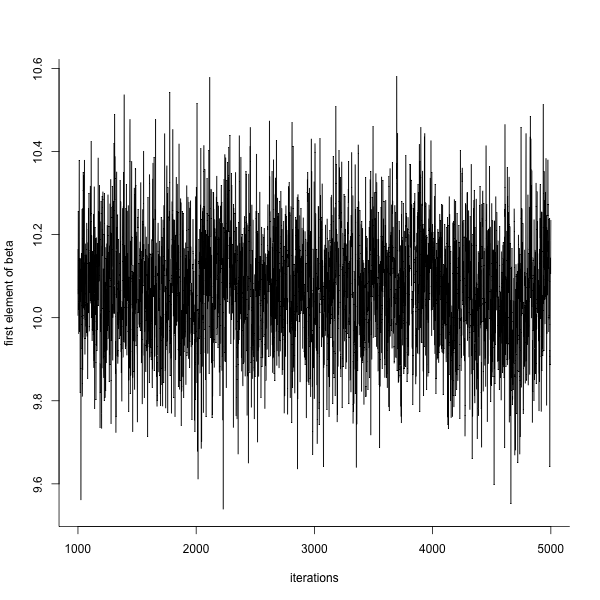
\includegraphics[width=\linewidth]{Ex5/figures/tra_beta.png} 
        %\caption{Competitors} \label{fig:timing2}
    \end{subfigure}

    \vspace{1cm}
    \centering
    \begin{subfigure}[t]{0.45\textwidth}
        \centering
        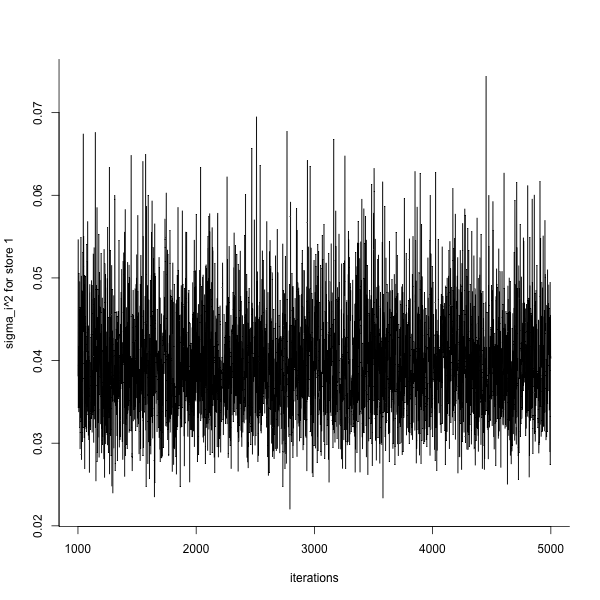
\includegraphics[width=\linewidth]{Ex5/figures/tra_sig2.png} 
        %\caption{Generic} \label{fig:timing1}
    \end{subfigure}
    \hfill
    \begin{subfigure}[t]{0.45\textwidth}
        \centering
        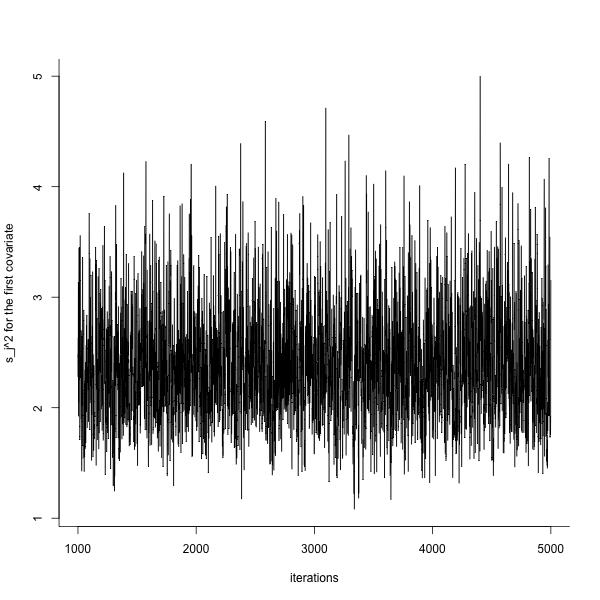
\includegraphics[width=\linewidth]{Ex5/figures/tra_s2.png} 
        %\caption{Competitors} \label{fig:timing2}
    \end{subfigure}
    \caption{Trace plots.}
\end{figure}


\clearpage \newpage
\section{A hierarchical probit model}

Read the following paper (or read some distillation of the paper in a book/blog post/slides/etc).  
\begin{quotation}
``Bayesian Analysis of Binary and Polychotomous Response Data.''  James H. Albert and Siddhartha Chib.  \textit{Journal of the American Statistical Association}, Vol.~88, No.~422 (Jun.,~1993), pp.~669-679
\end{quotation}

The paper describes a Bayesian treatment of probit regression (similar to logistic regression) using the trick of \textit{data augmentation}---that is, introducing ``latent variables'' that turn a hard problem into a much easier one.  Briefly summarize your understanding of the key trick proposed by this paper.  Then see you if you can apply the trick in the following context, which is more complex than ordinary probit regression.

In ``polls.csv'' you will find the results of several political polls from the 1988 U.S.~presidential election.  The outcome of interest is whether someone plans to vote for George Bush (senior, not junior).  There are several potentially relevant demographic predictors here, including the respondent's state of residence.  The goal is to understand how these relate to the probability that someone will support Bush in the election.  You can imagine this information would help a great deal in poll re-weighting and aggregation (ala Nate Silver).

Use Gibbs sampling, together with the Albert and Chib trick, to fit a hierarchical probit model of the following form:
\begin{eqnarray*}
\mbox{Pr}(y_{ij} = 1) &=& \Phi(z_{ij})  \\
z_{ij} &=& \mu_i + x_{ij}^T \beta_i \, .
\end{eqnarray*}
Here $y_{ij}$ is the response (Bush=1, other=0) for respondent $j$ in state $i$; $\Phi(\cdot)$ is the probit link function, i.e.~the CDF of the standard normal distribution; $\mu_i$ is a state-level intercept term; $x_{ij}$ is a vector of respondent-level demographic predictors; and $\beta_i$ is a vector of regression coefficients for state $i$.

Notes:
\begin{enumerate}
\item There are severe imbalances among the states in terms of numbers of survey respondents. Following the last problem, the key is to impose a hierarchical prior on the state-level parameters.
\item The data-augmentation trick from the Albert and Chib paper above is explained in many standard references on Bayesian analysis.  If you want to get a quick introduction to the idea, you can consult one of these.  A good presentation is in Section 8.1.1 of ``Bayesian analysis for the social sciences'' by Simon Jackman, available as an ebook through lib.utexas.edu.
\item You are welcome to use the logit model instead of the probit model.  If you do this, you'll need to read the following paper, rather than Albert and Chib: Polson, N.G., Scott, J.G. and Windle, J. (2013). Bayesian inference for logistic models using Polya-Gamma latent variables. J. Amer. Statist. Assoc. 108 1339--1349.    You can find a routine for simulation Polya-Gamma random variables in the BayesLogit R package and the pypolyagamma python library.  
\end{enumerate}

\bigskip \jie
The basic idea of the reference paper is that for models like probit model, we can use data augmentation to use MCMC algorithim to sample from the posterior. Adding some hidden variable may make the inference easier.

The model I am using to solve this problem is as follows.

Likelihood:
\begin{eqnarray*}
\mbox{Pr}(y_{ij} = 1) &=& \Phi(z_{ij})  \\
z_{ij} &=& \mu_i + x_{ij}^T \beta_i \, 
\end{eqnarray*}
rewrite this as (change notation for convenience)
$$z_{ij} = x_{ij}^T \beta_i$$

Priors:
\begin{align*}
    \beta_i &\sim N(\mu, \Sigma = diag(\sigma_1^2, \dots, \sigma_p^2)) \\
    \sigma_k^2 &\sim \text{Inv-Ga}(\frac{1}2, \frac{1}2) \\
    \mu &\propto 1
\end{align*}

We can use the following data augmentation:
\begin{align*}
    a_{ij} &\sim N(x_{ij}^T \beta_i, 1) \\
    y_{ij} &= 1(a_{ij} >0)
\end{align*}

The full conditionals for Gibbs sampling are:
$$p(\beta_i \mid - ) \propto N(\tilde{\mu}_i, \tilde{\Sigma}_i),$$
where
$$\tilde{\Sigma}_i = (X_i^TX_i + \Sigma^{-1})^{-1}, \;\; \tilde{\mu}_i = \tilde{\Sigma}_i (X_i^Ta_i + \Sigma^{-1}\mu).$$
$$p(\mu \mid -) = N(\bar{\beta}, \frac{1}{n} \Sigma).$$
$$p(\sigma_k^2 \mid -) = \text{Inv-Ga}(\frac{1}2 + \frac{1}n, \frac{1}2 + \frac{1}2 \sum_{i=1}^n (\beta_{ik} - \mu_k)^2 ).$$
$$p(a_{ij} \mid -) = N(a_{ij} \mid x_{ij}^T\beta_i, 1) 
\begin{cases}
1(a_{ij} >0), & y_{ij}=1 \\
1(a_{ij} \leq 0), & y_{ij}=0 
\end{cases}$$

\begin{figure}
    \centering
    \begin{subfigure}[t]{0.9\textwidth}
        \centering
        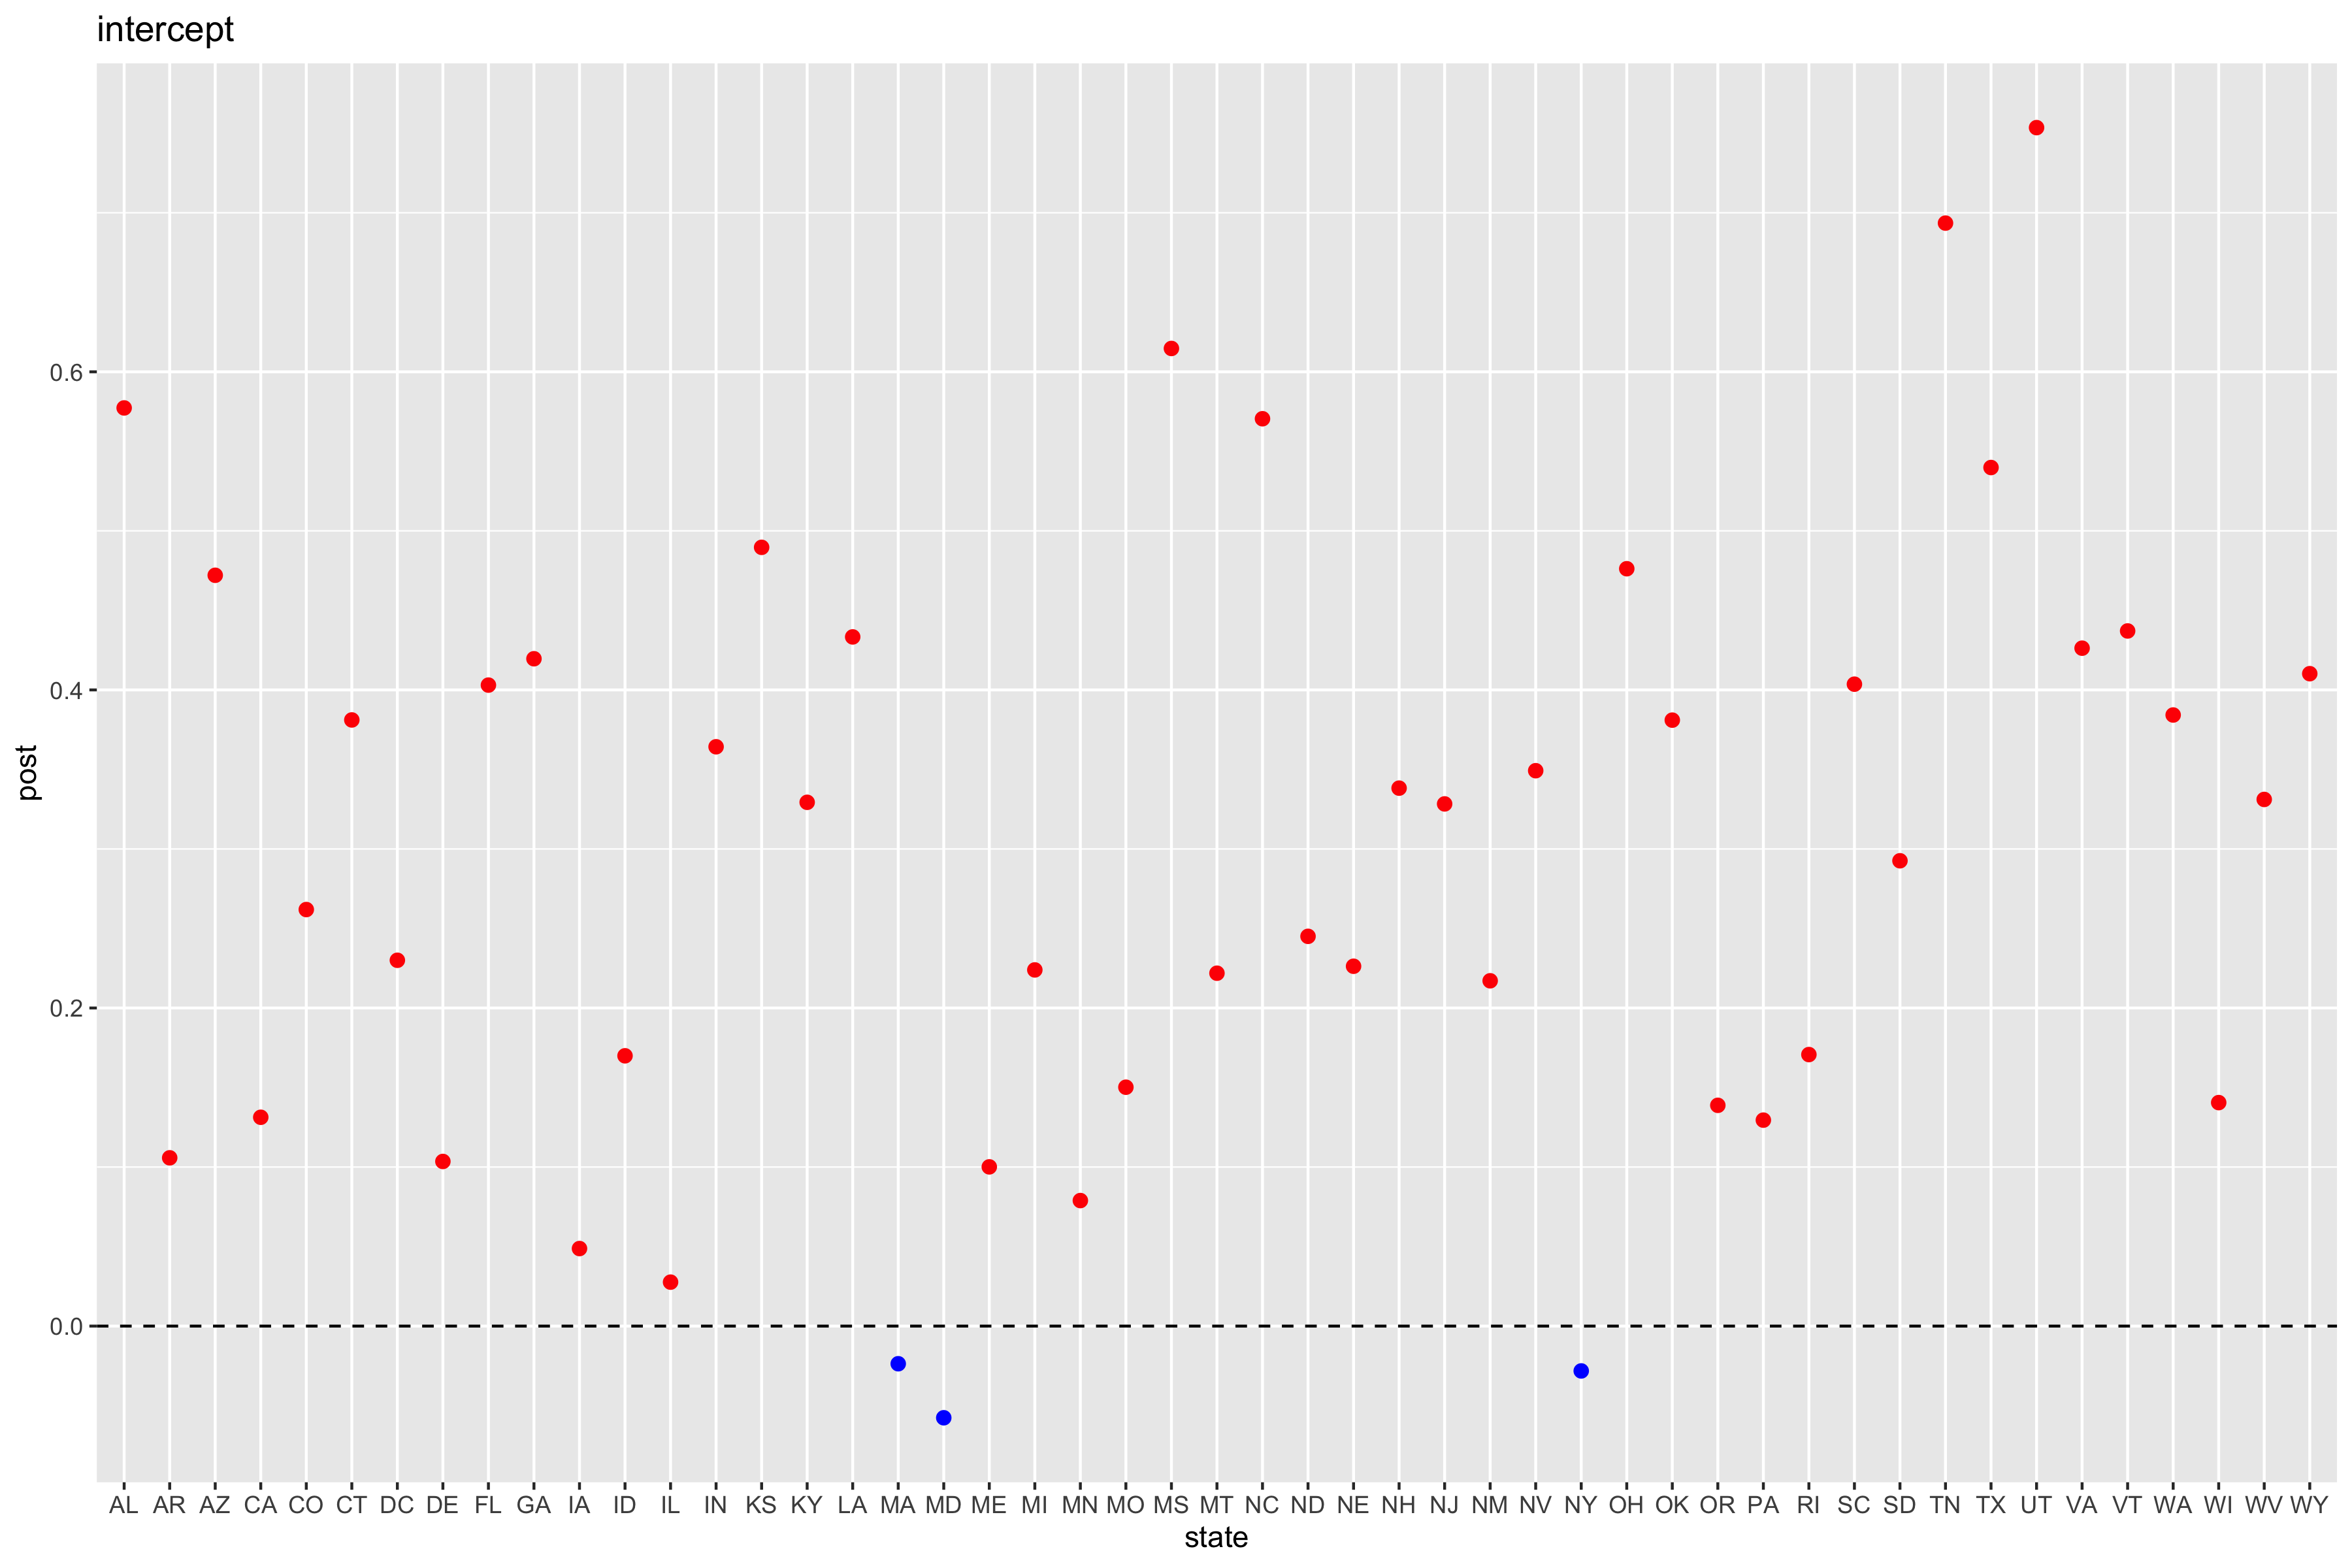
\includegraphics[width=\linewidth]{Ex5/figures/2post covariates1.png} 
        %\caption{Generic} \label{fig:timing1}
    \end{subfigure}
    \hfill
    \begin{subfigure}[t]{0.9\textwidth}
        \centering
        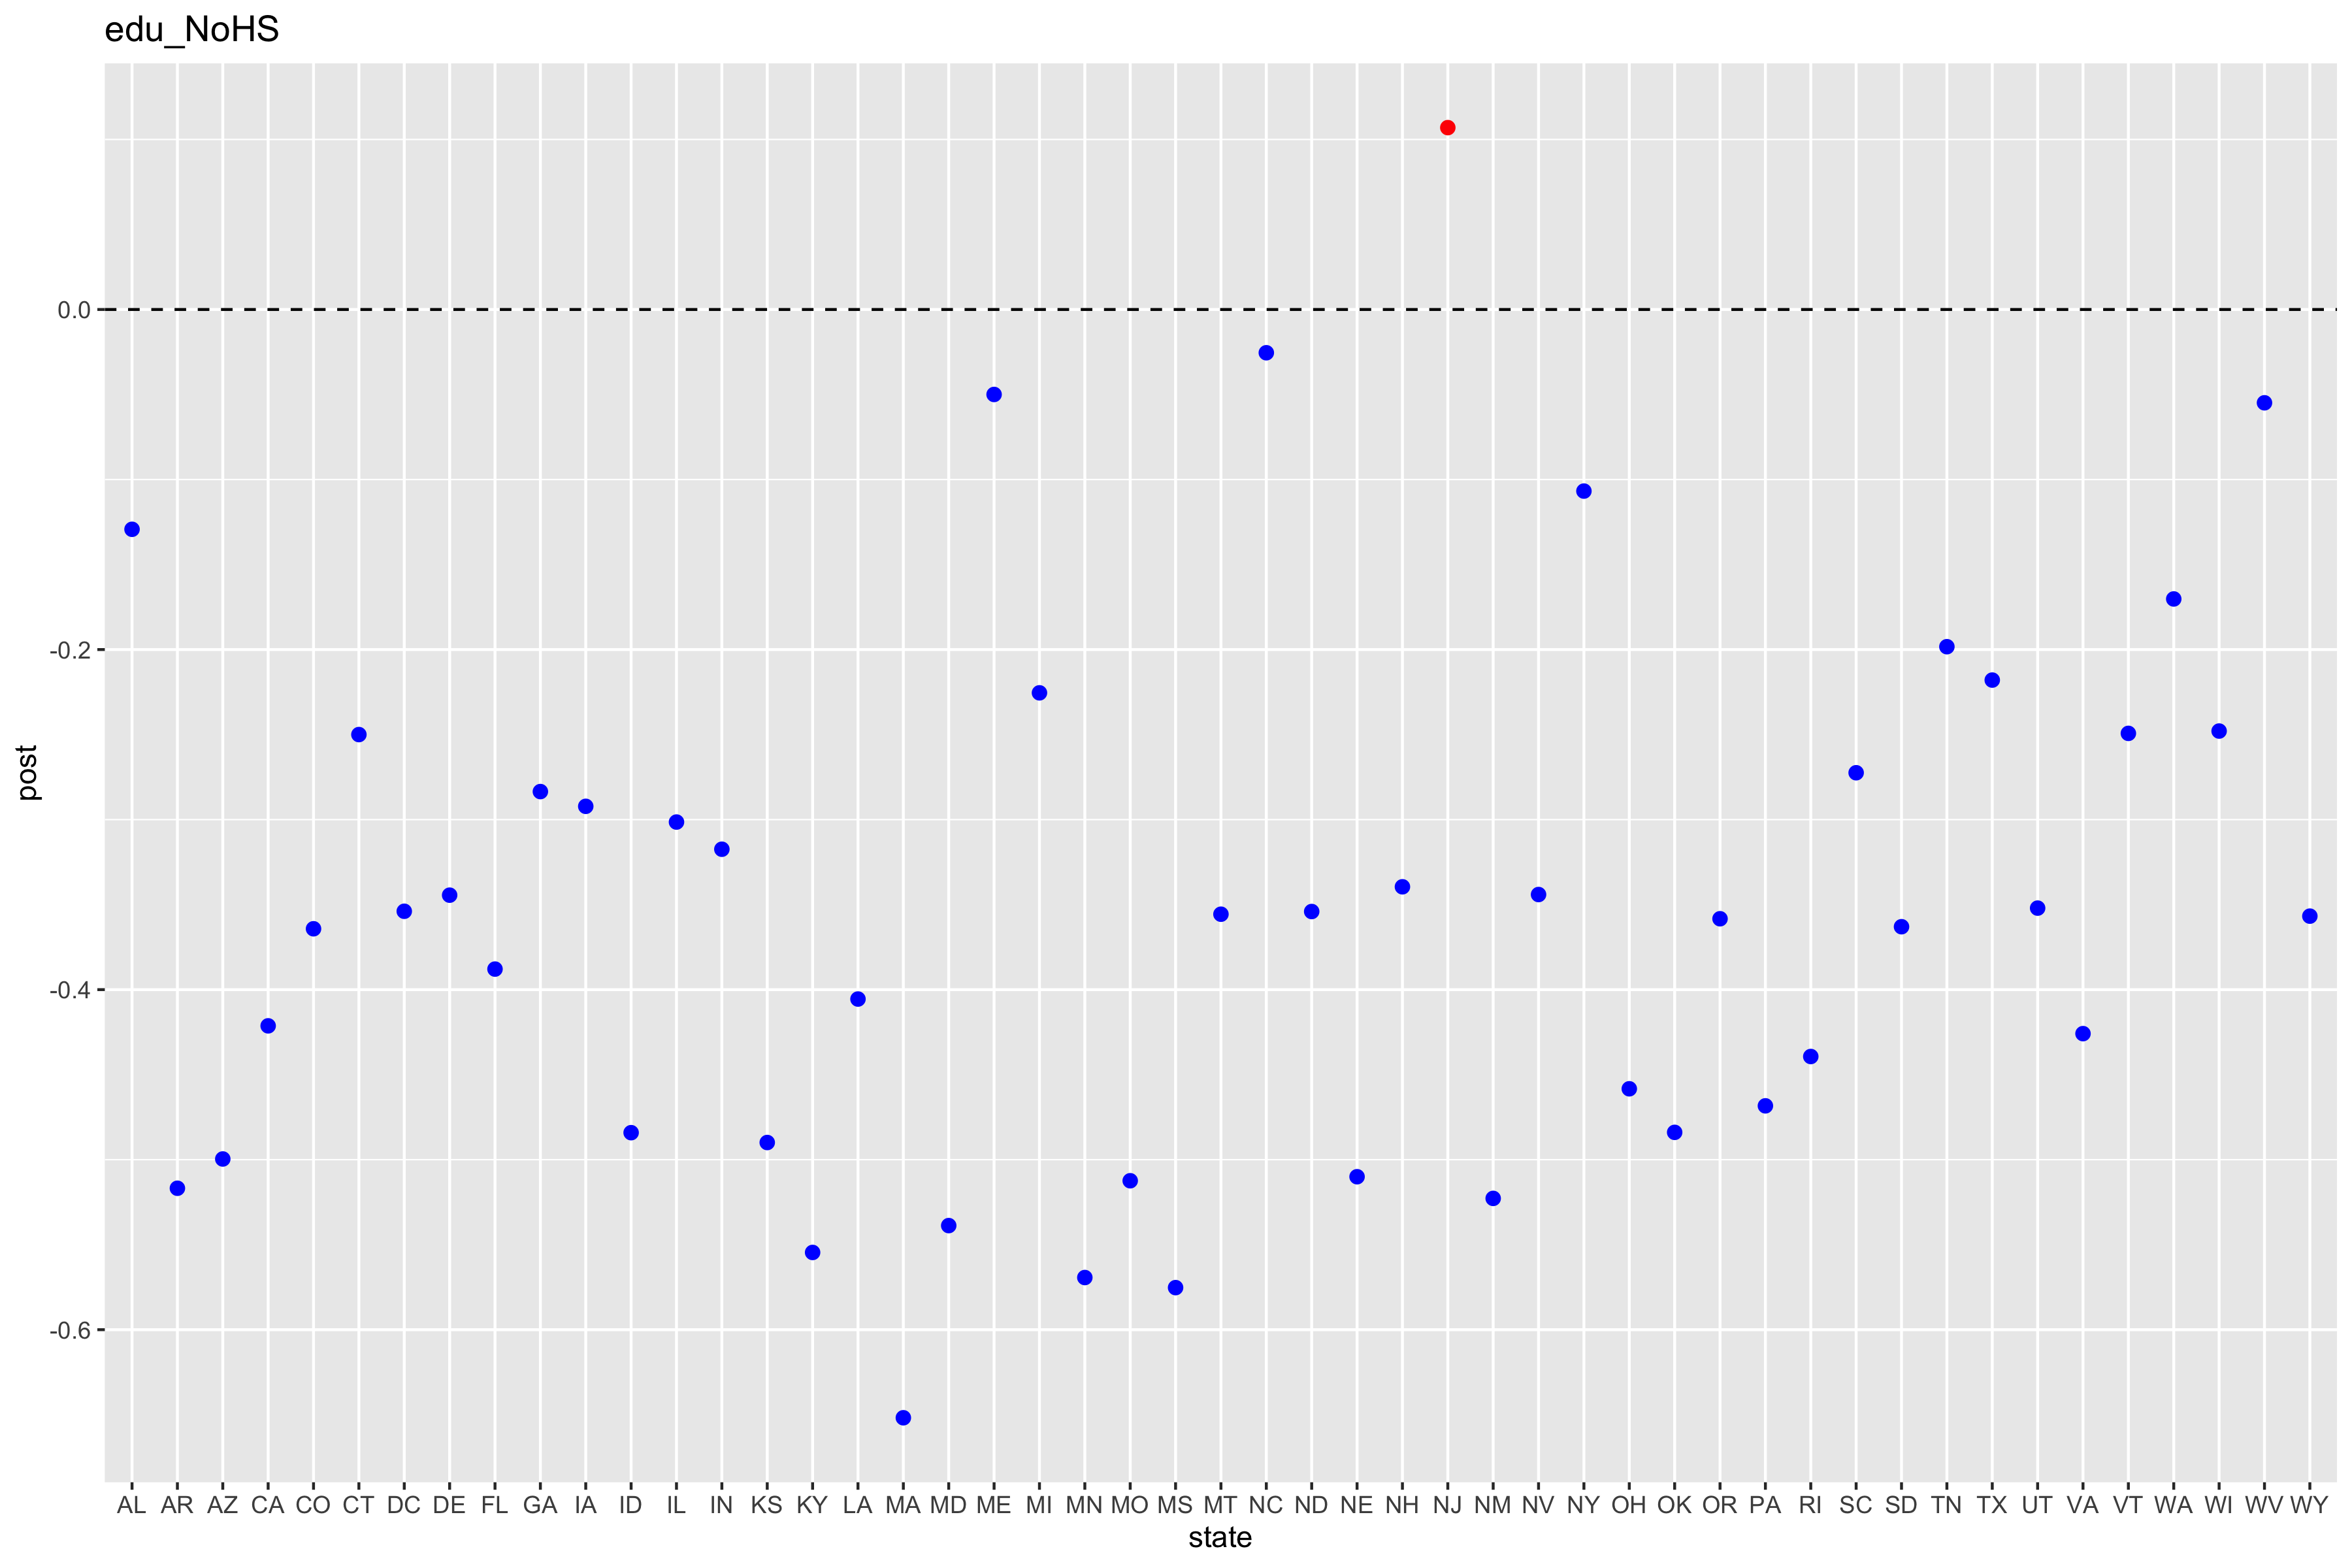
\includegraphics[width=\linewidth]{Ex5/figures/2post covariates2.png} 
        %\caption{Competitors} \label{fig:timing2}
    \end{subfigure}
\end{figure}

\begin{figure}

    \centering
    \begin{subfigure}[t]{0.9\textwidth}
        \centering
        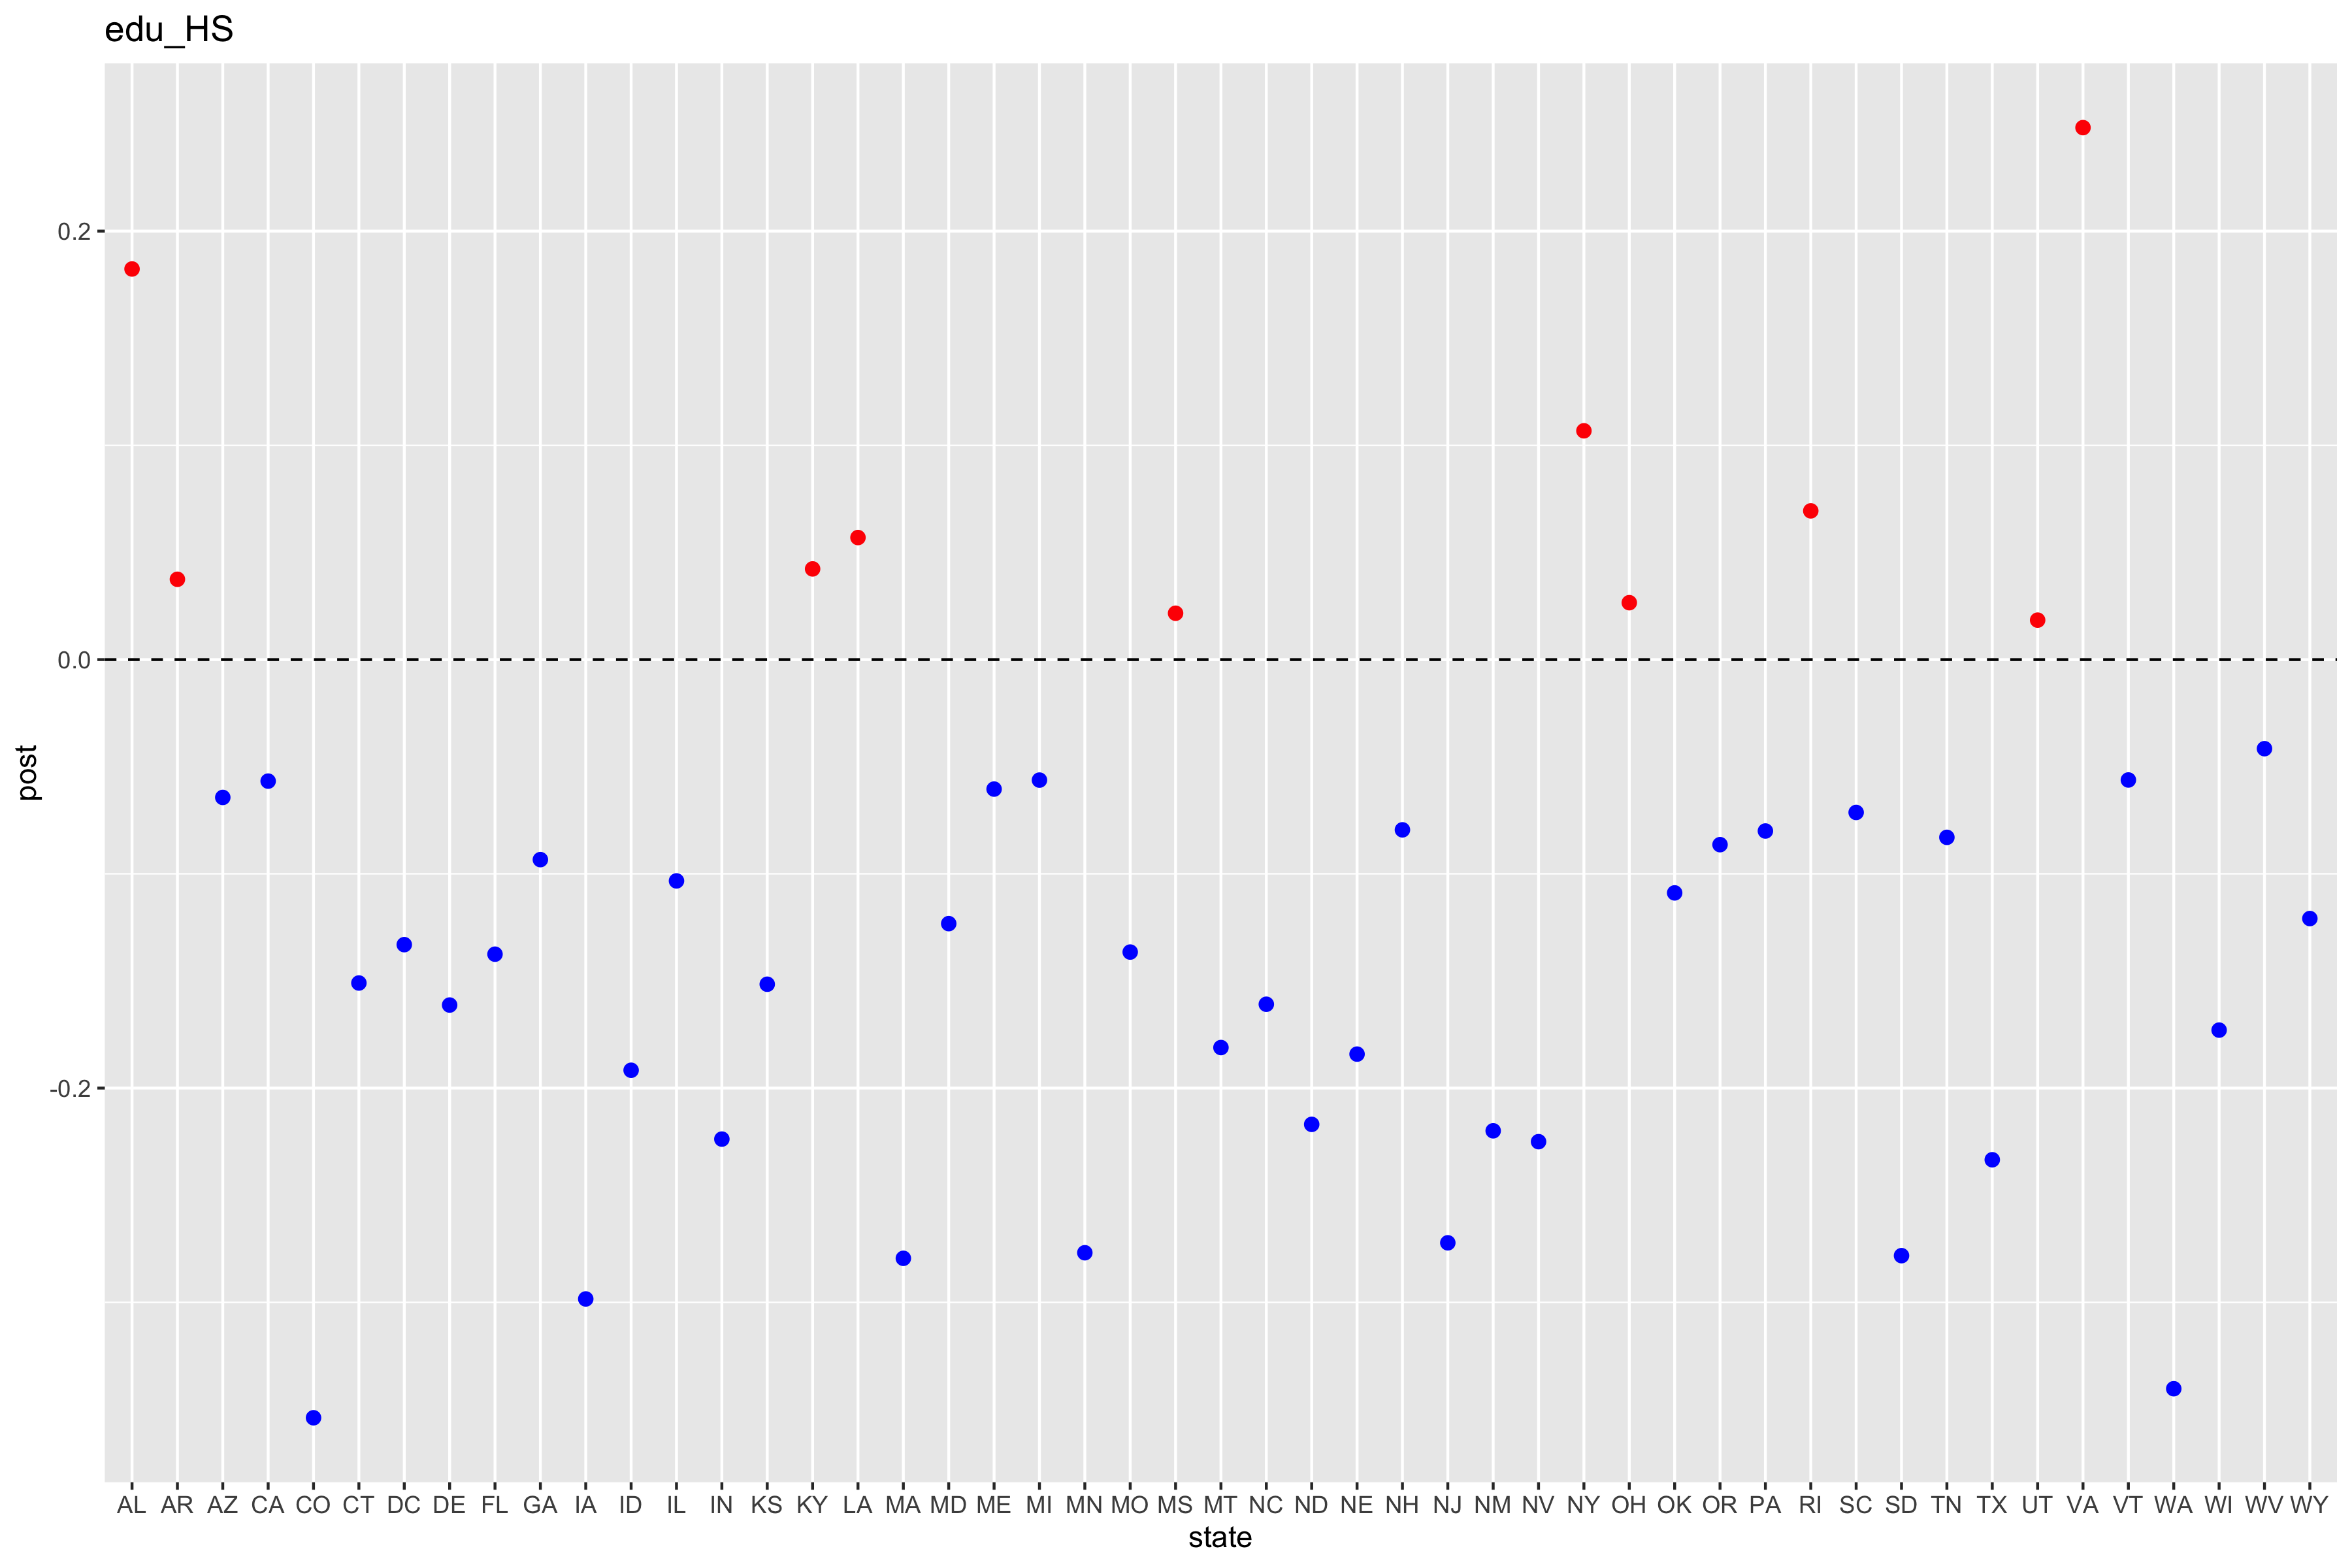
\includegraphics[width=\linewidth]{Ex5/figures/2post covariates3.png} 
        %\caption{Generic} \label{fig:timing1}
    \end{subfigure}
    \hfill
    \begin{subfigure}[t]{0.9\textwidth}
        \centering
        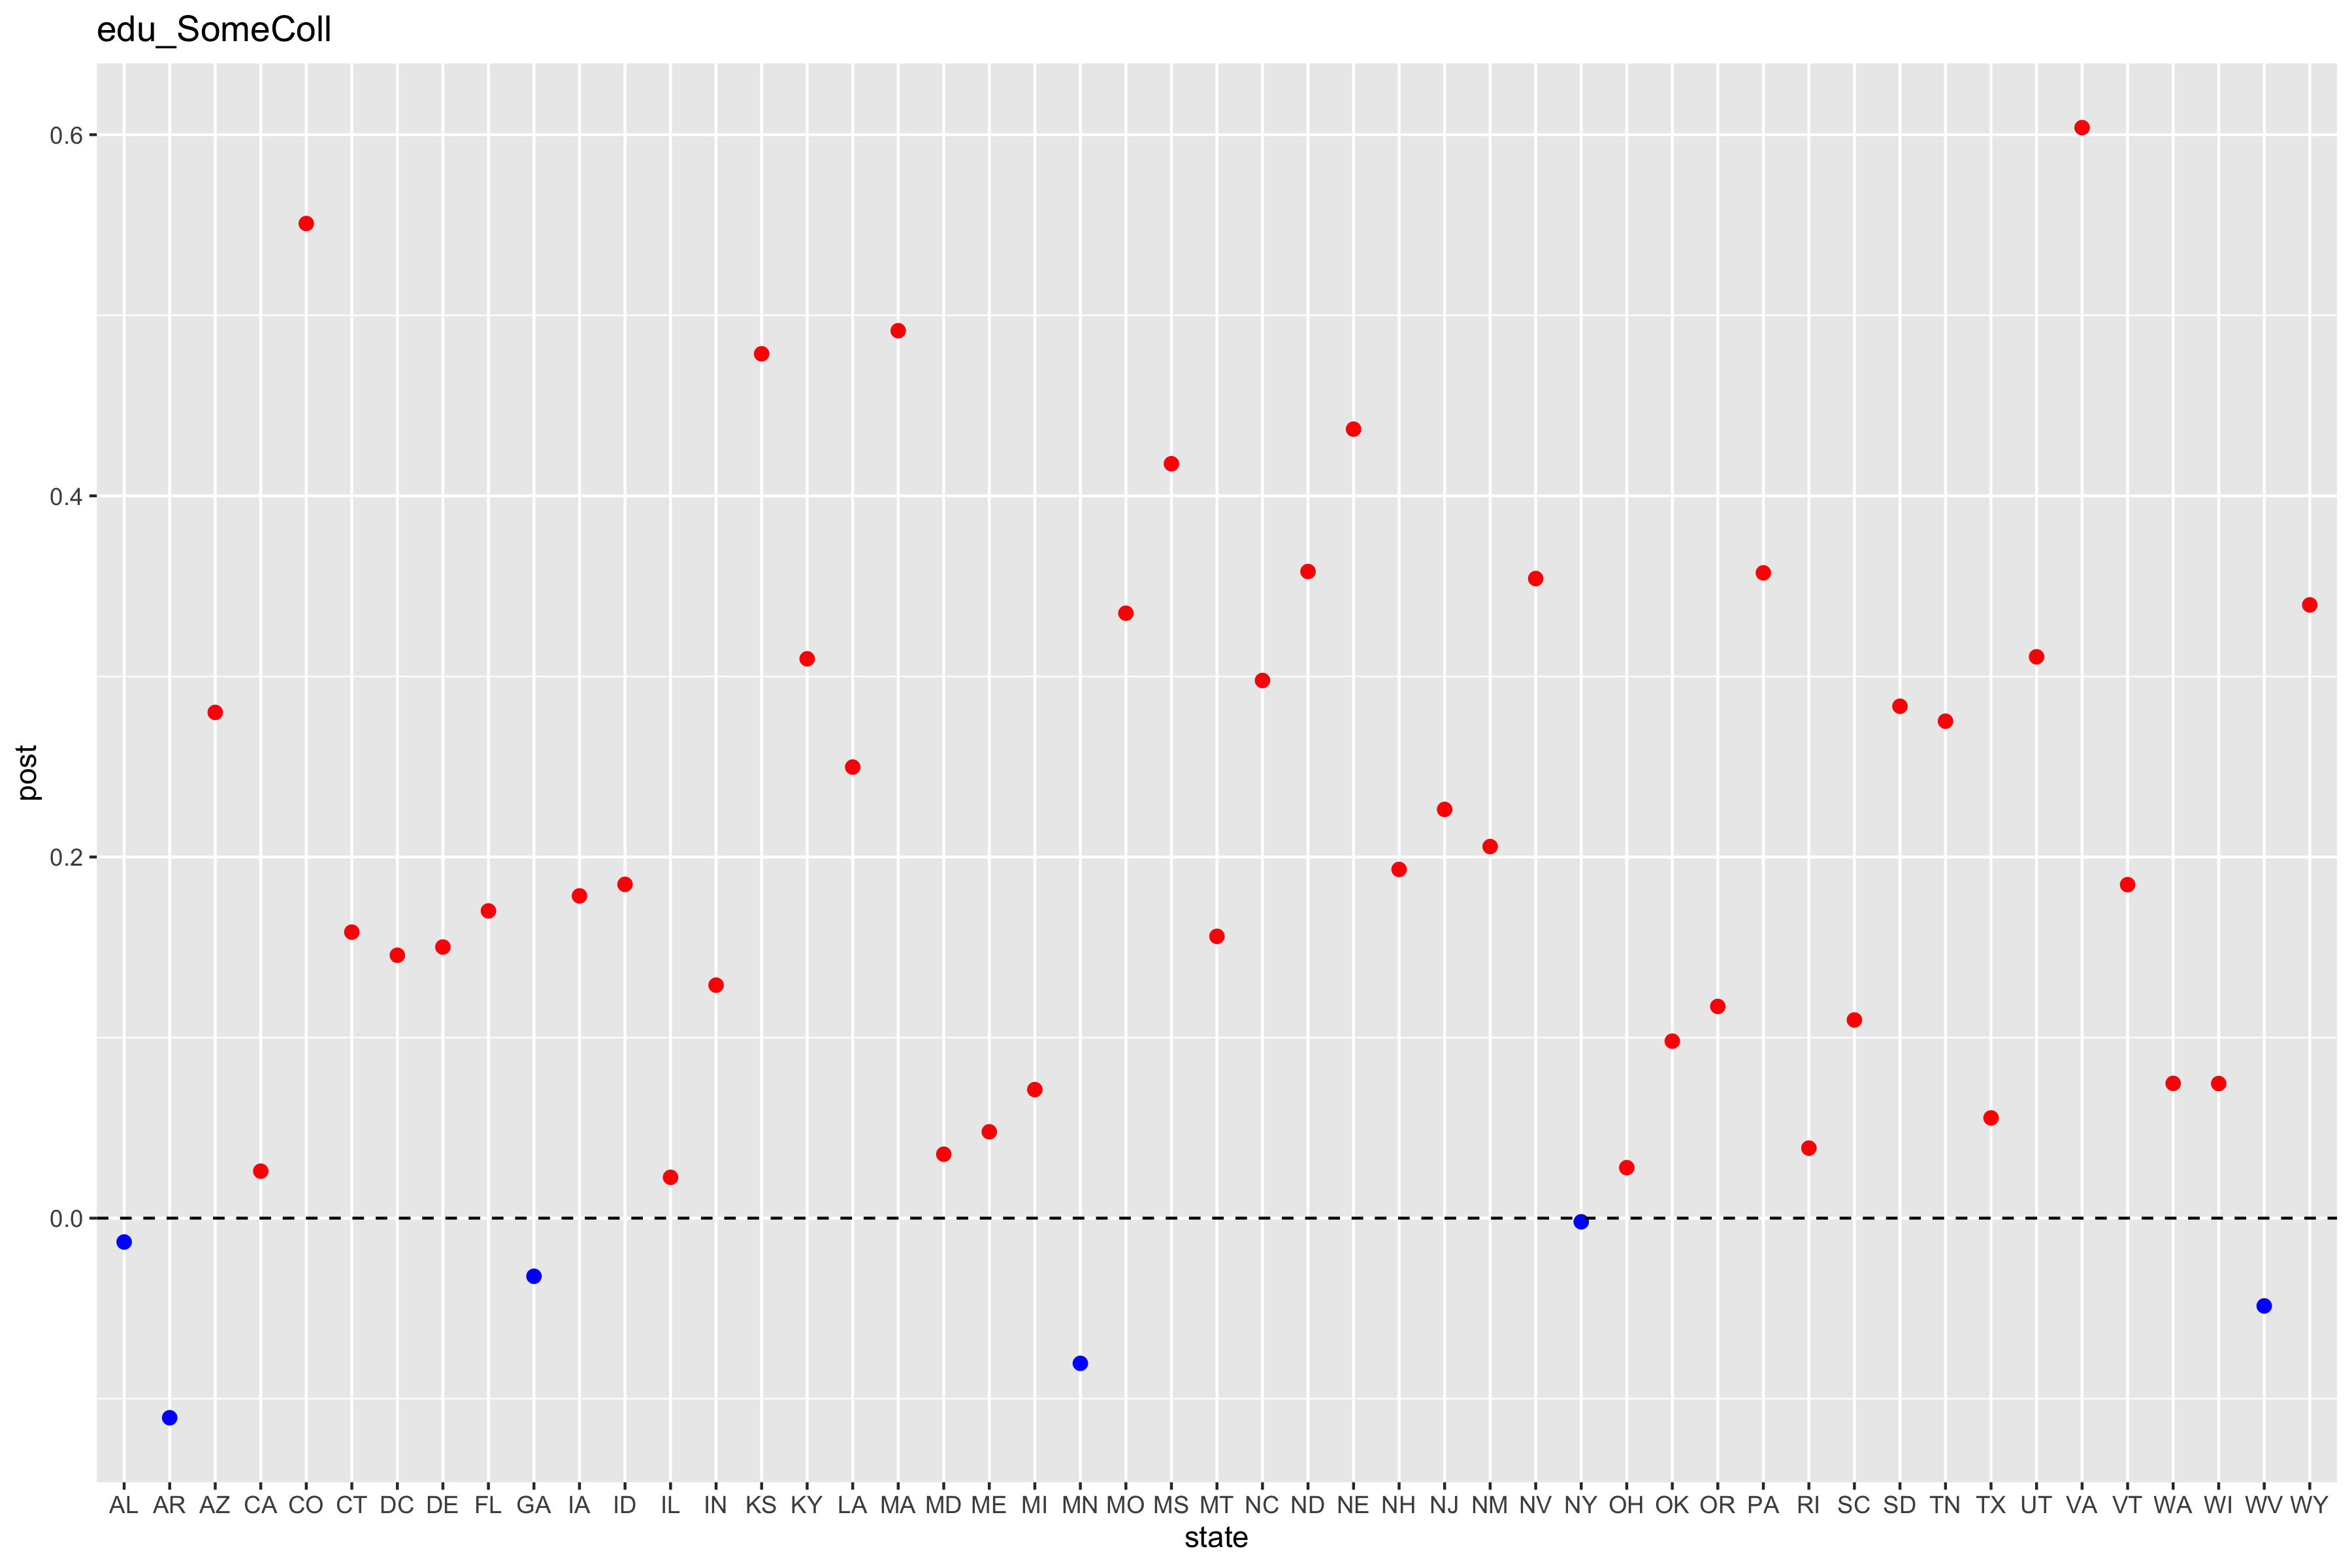
\includegraphics[width=\linewidth]{Ex5/figures/2post covariates4.png} 
        %\caption{Competitors} \label{fig:timing2}
    \end{subfigure}
    %\caption{Posterior estimates of the covariates.}
\end{figure}

\begin{figure}
    \centering
    \begin{subfigure}[t]{0.9\textwidth}
        \centering
        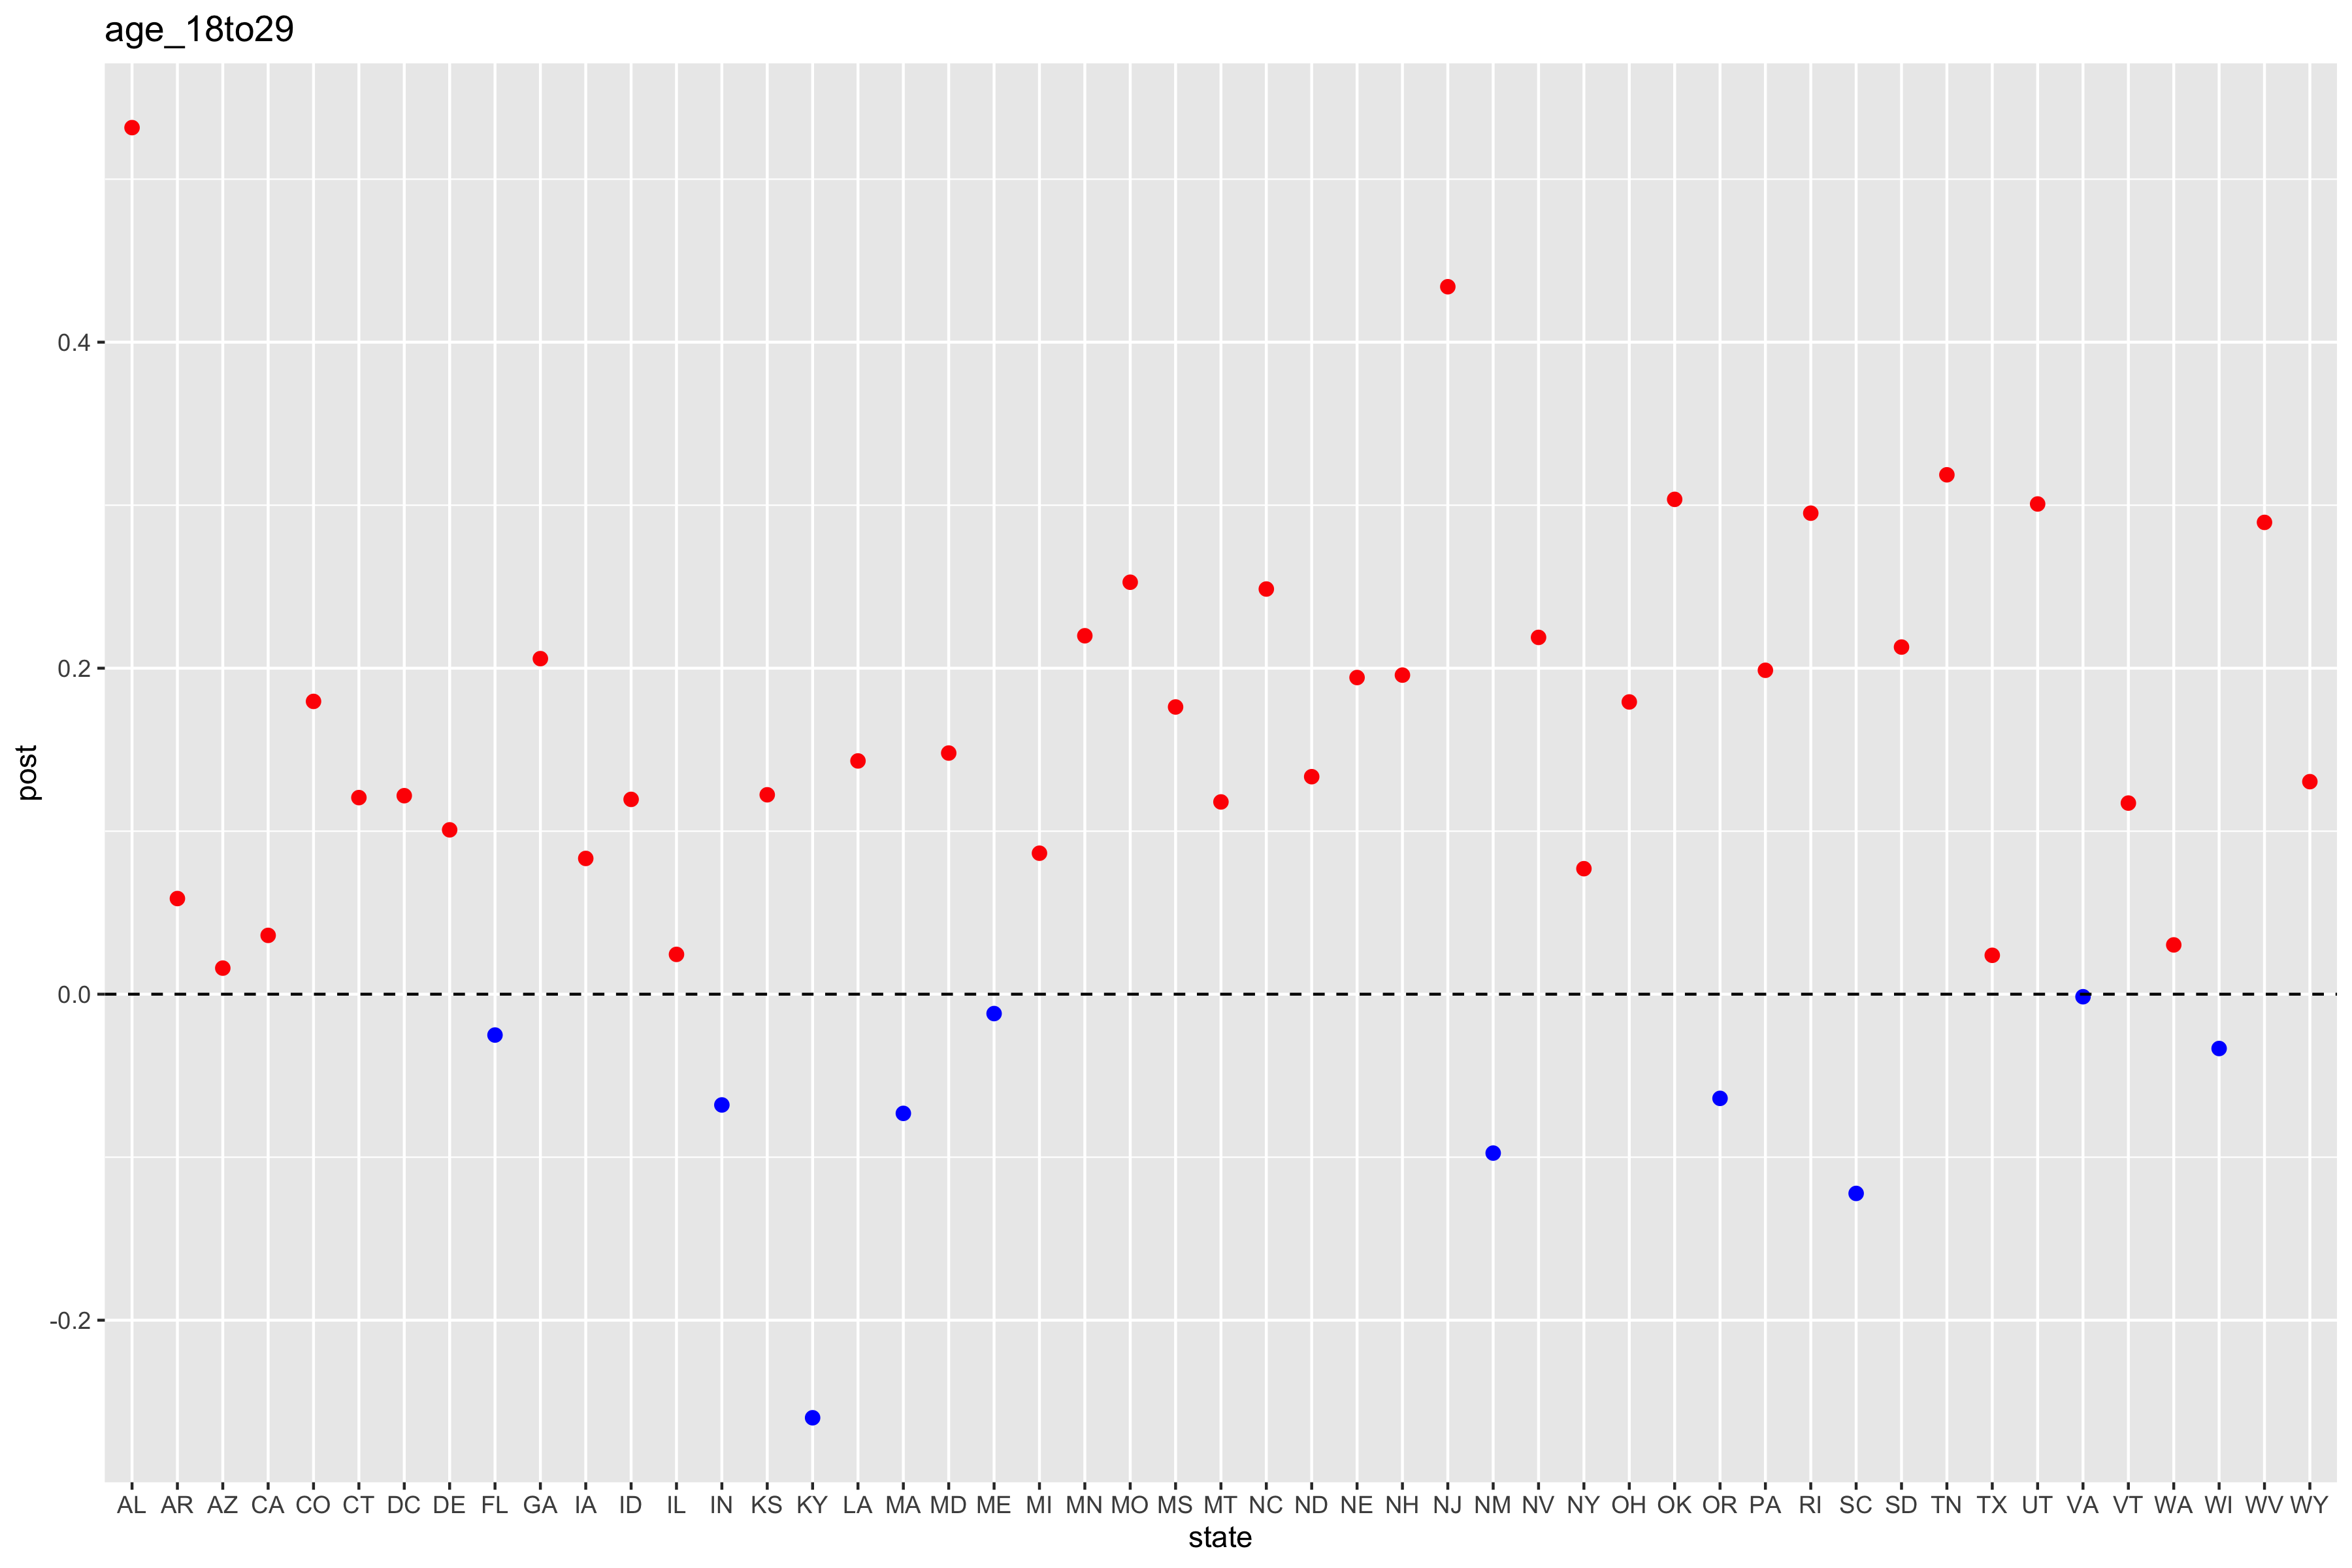
\includegraphics[width=\linewidth]{Ex5/figures/2post covariates5.png} 
        %\caption{Generic} \label{fig:timing1}
    \end{subfigure}
    \hfill
    \begin{subfigure}[t]{0.9\textwidth}
        \centering
        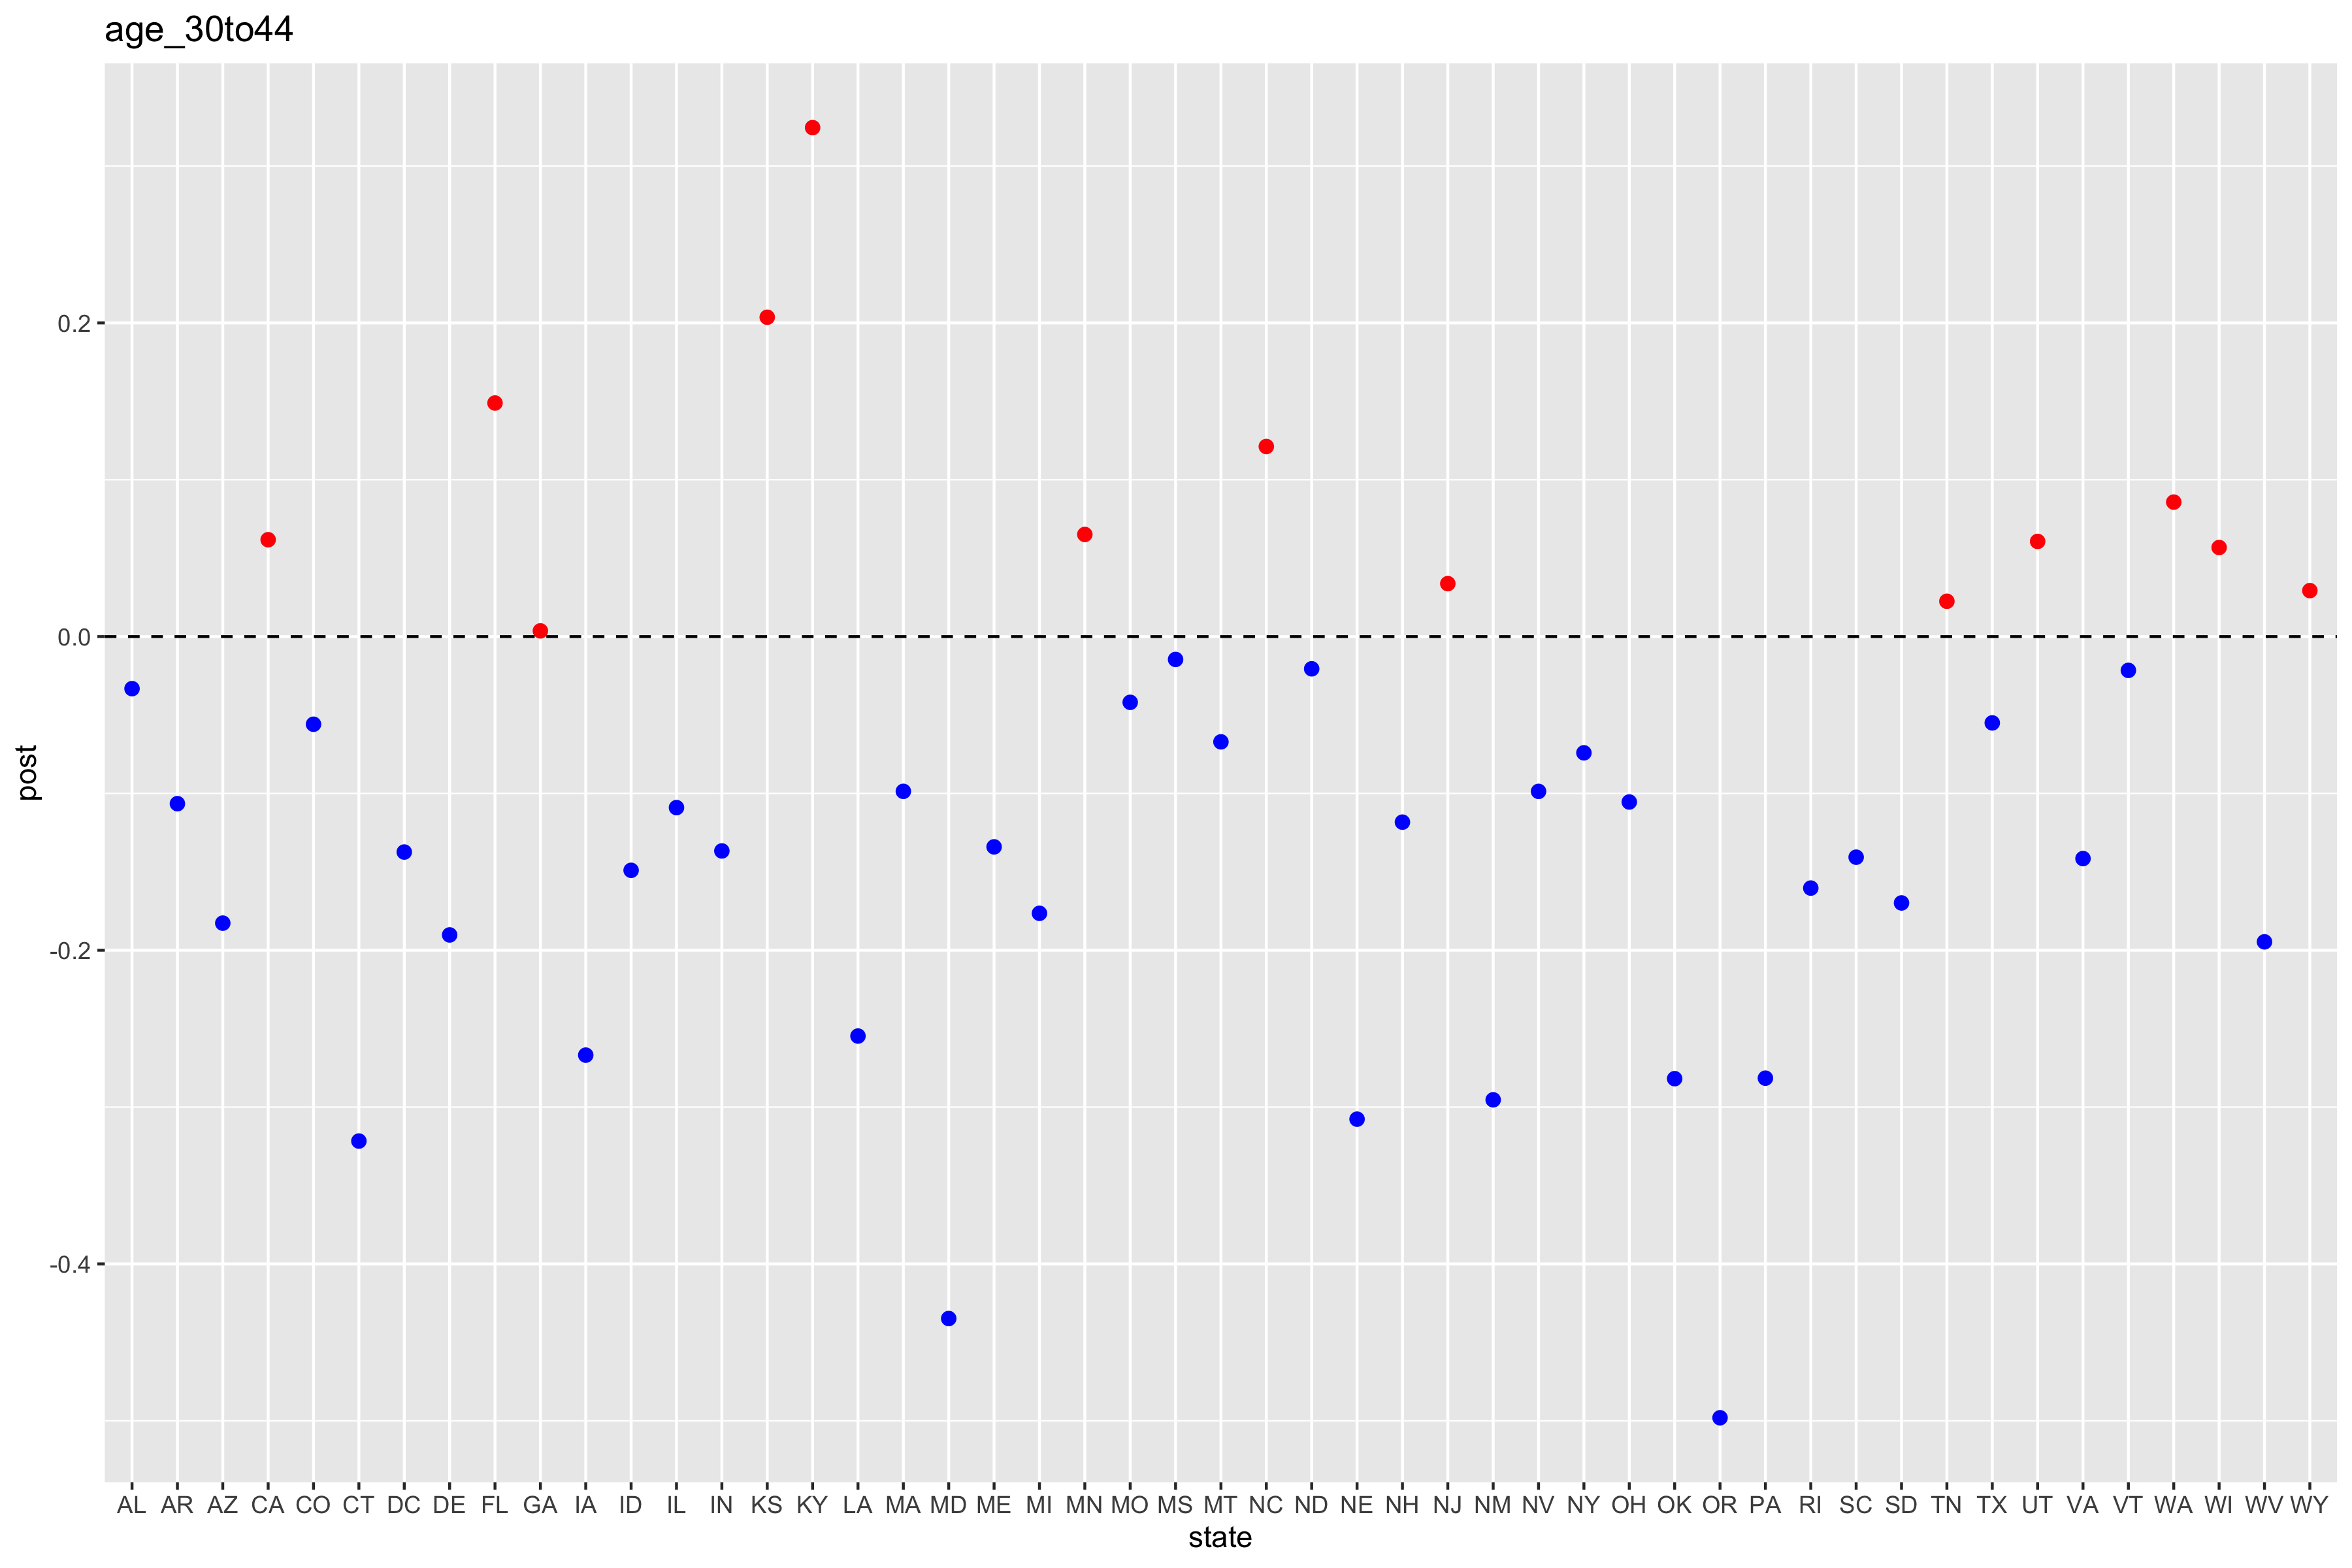
\includegraphics[width=\linewidth]{Ex5/figures/2post covariates6.png} 
        %\caption{Competitors} \label{fig:timing2}
    \end{subfigure}
\end{figure}

\begin{figure}

    \centering
    \begin{subfigure}[t]{0.9\textwidth}
        \centering
        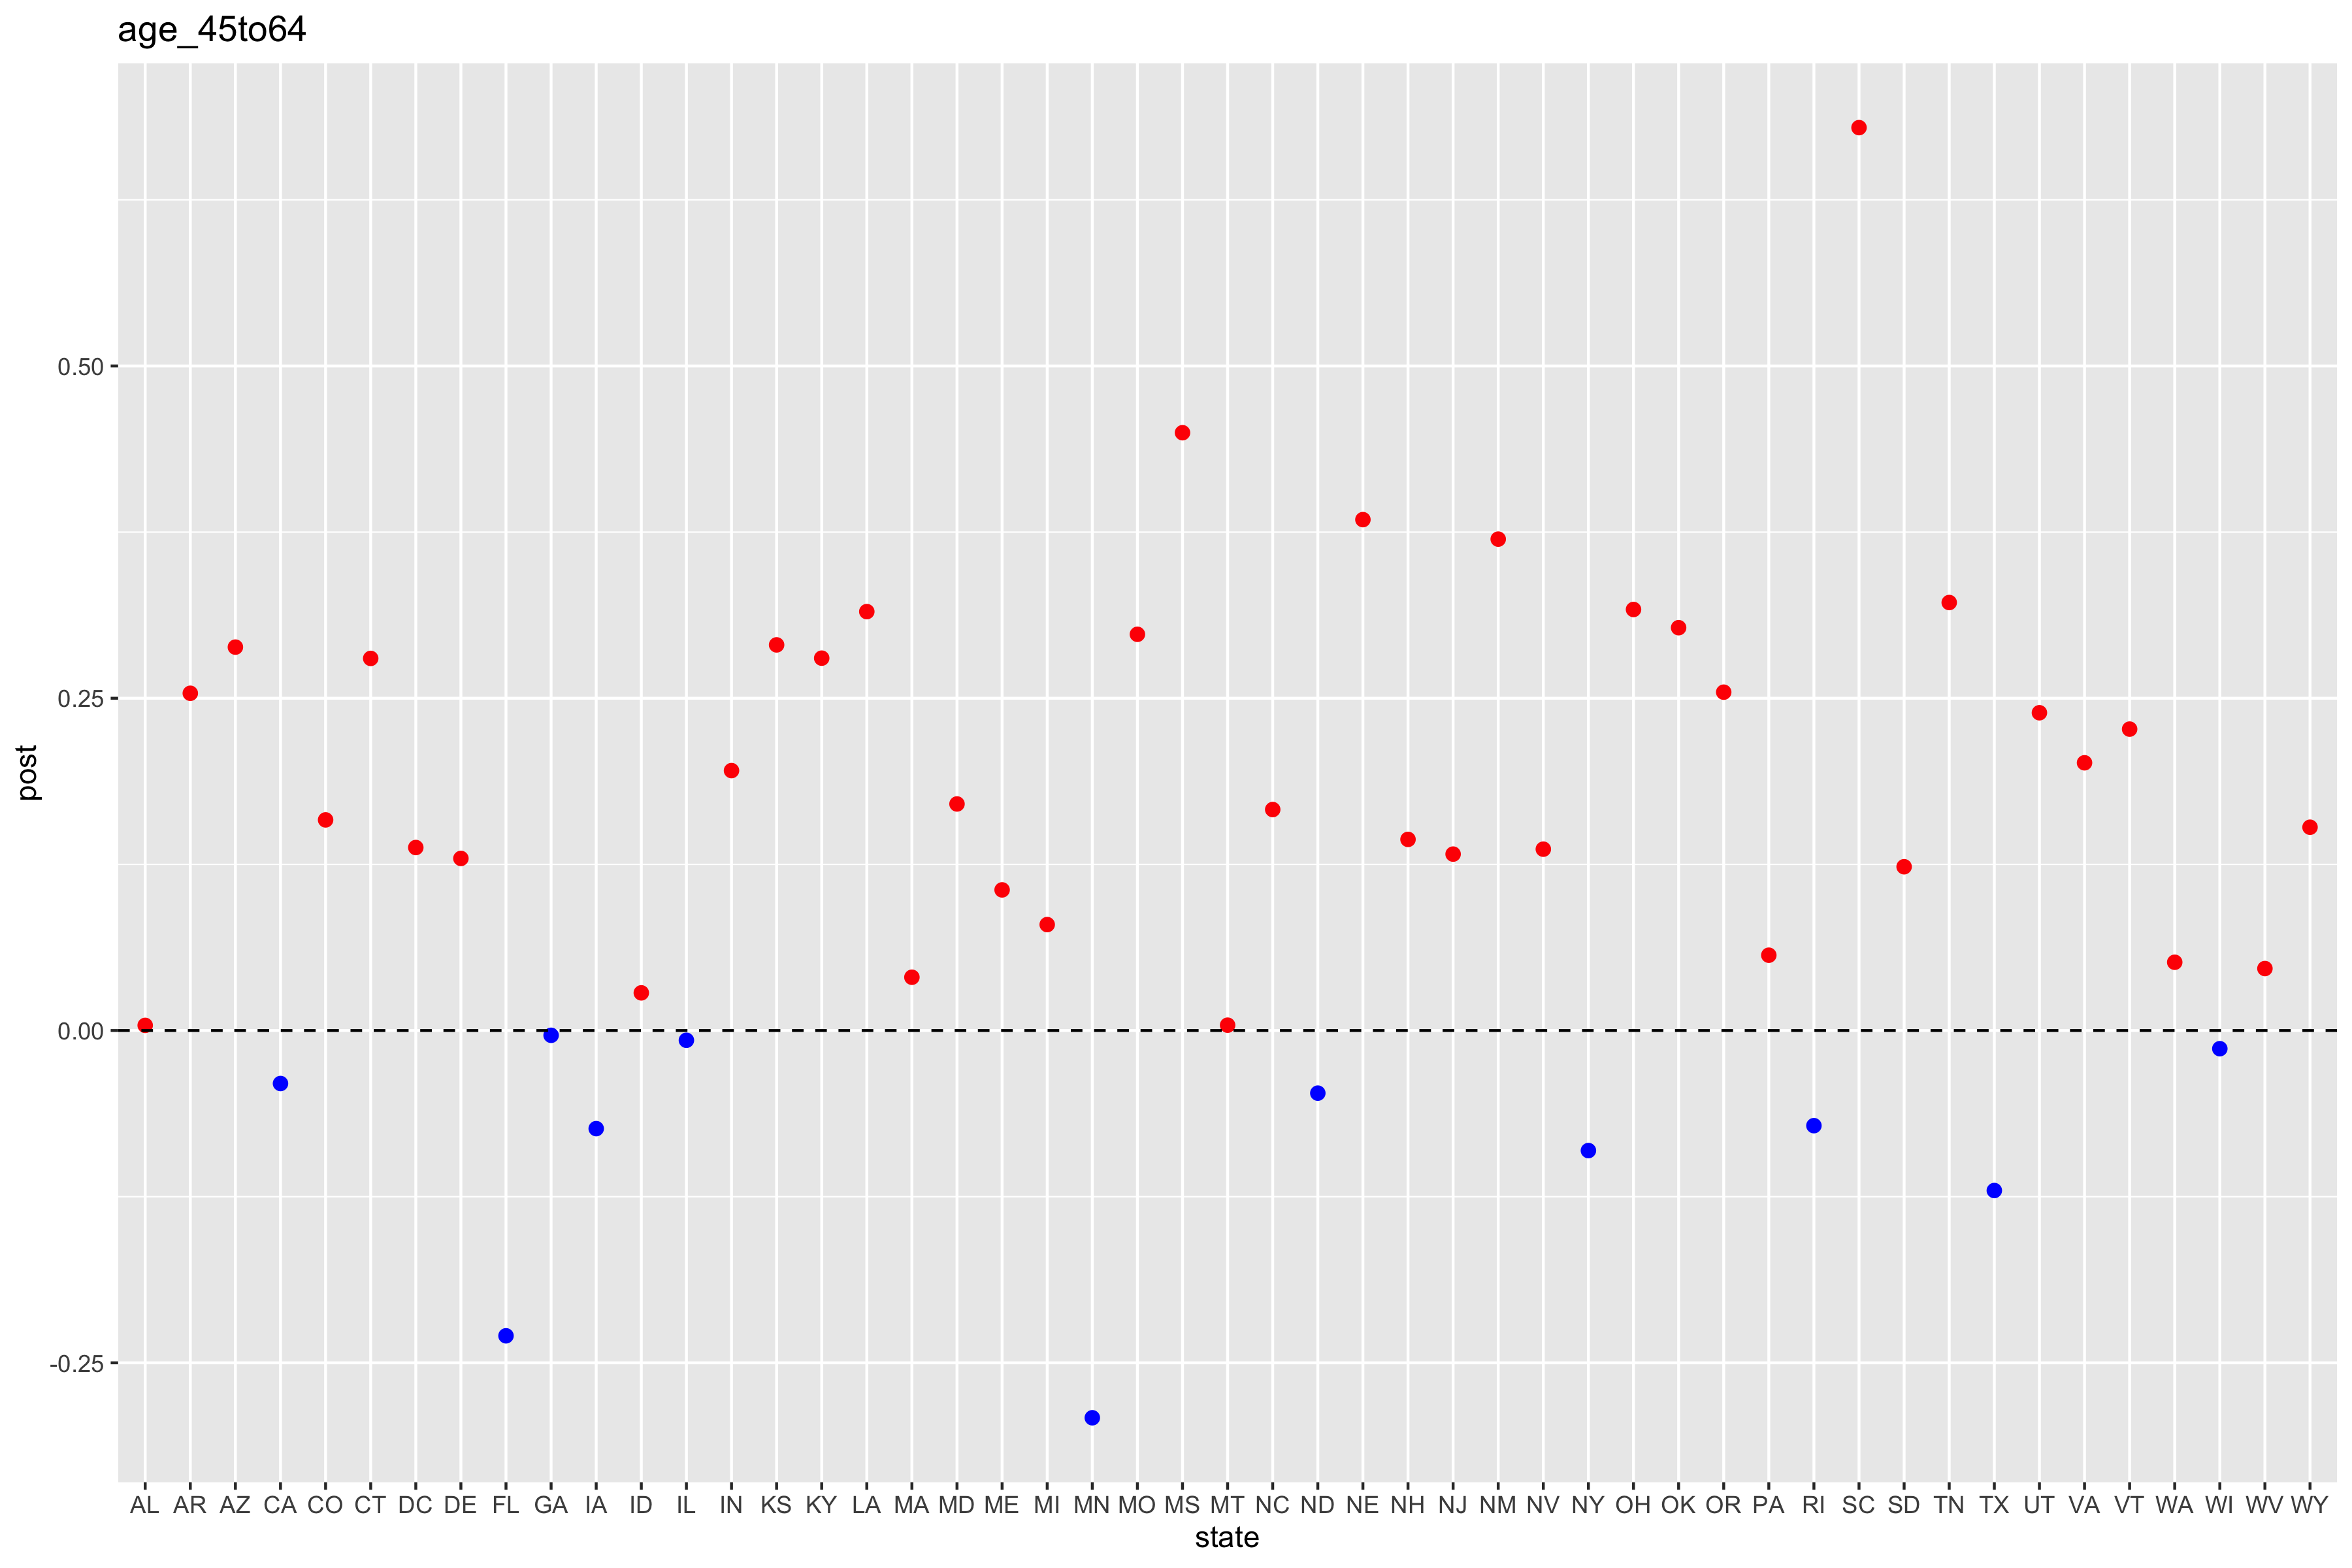
\includegraphics[width=\linewidth]{Ex5/figures/2post covariates7.png} 
        %\caption{Generic} \label{fig:timing1}
    \end{subfigure}
    \hfill
    \begin{subfigure}[t]{0.9\textwidth}
        \centering
        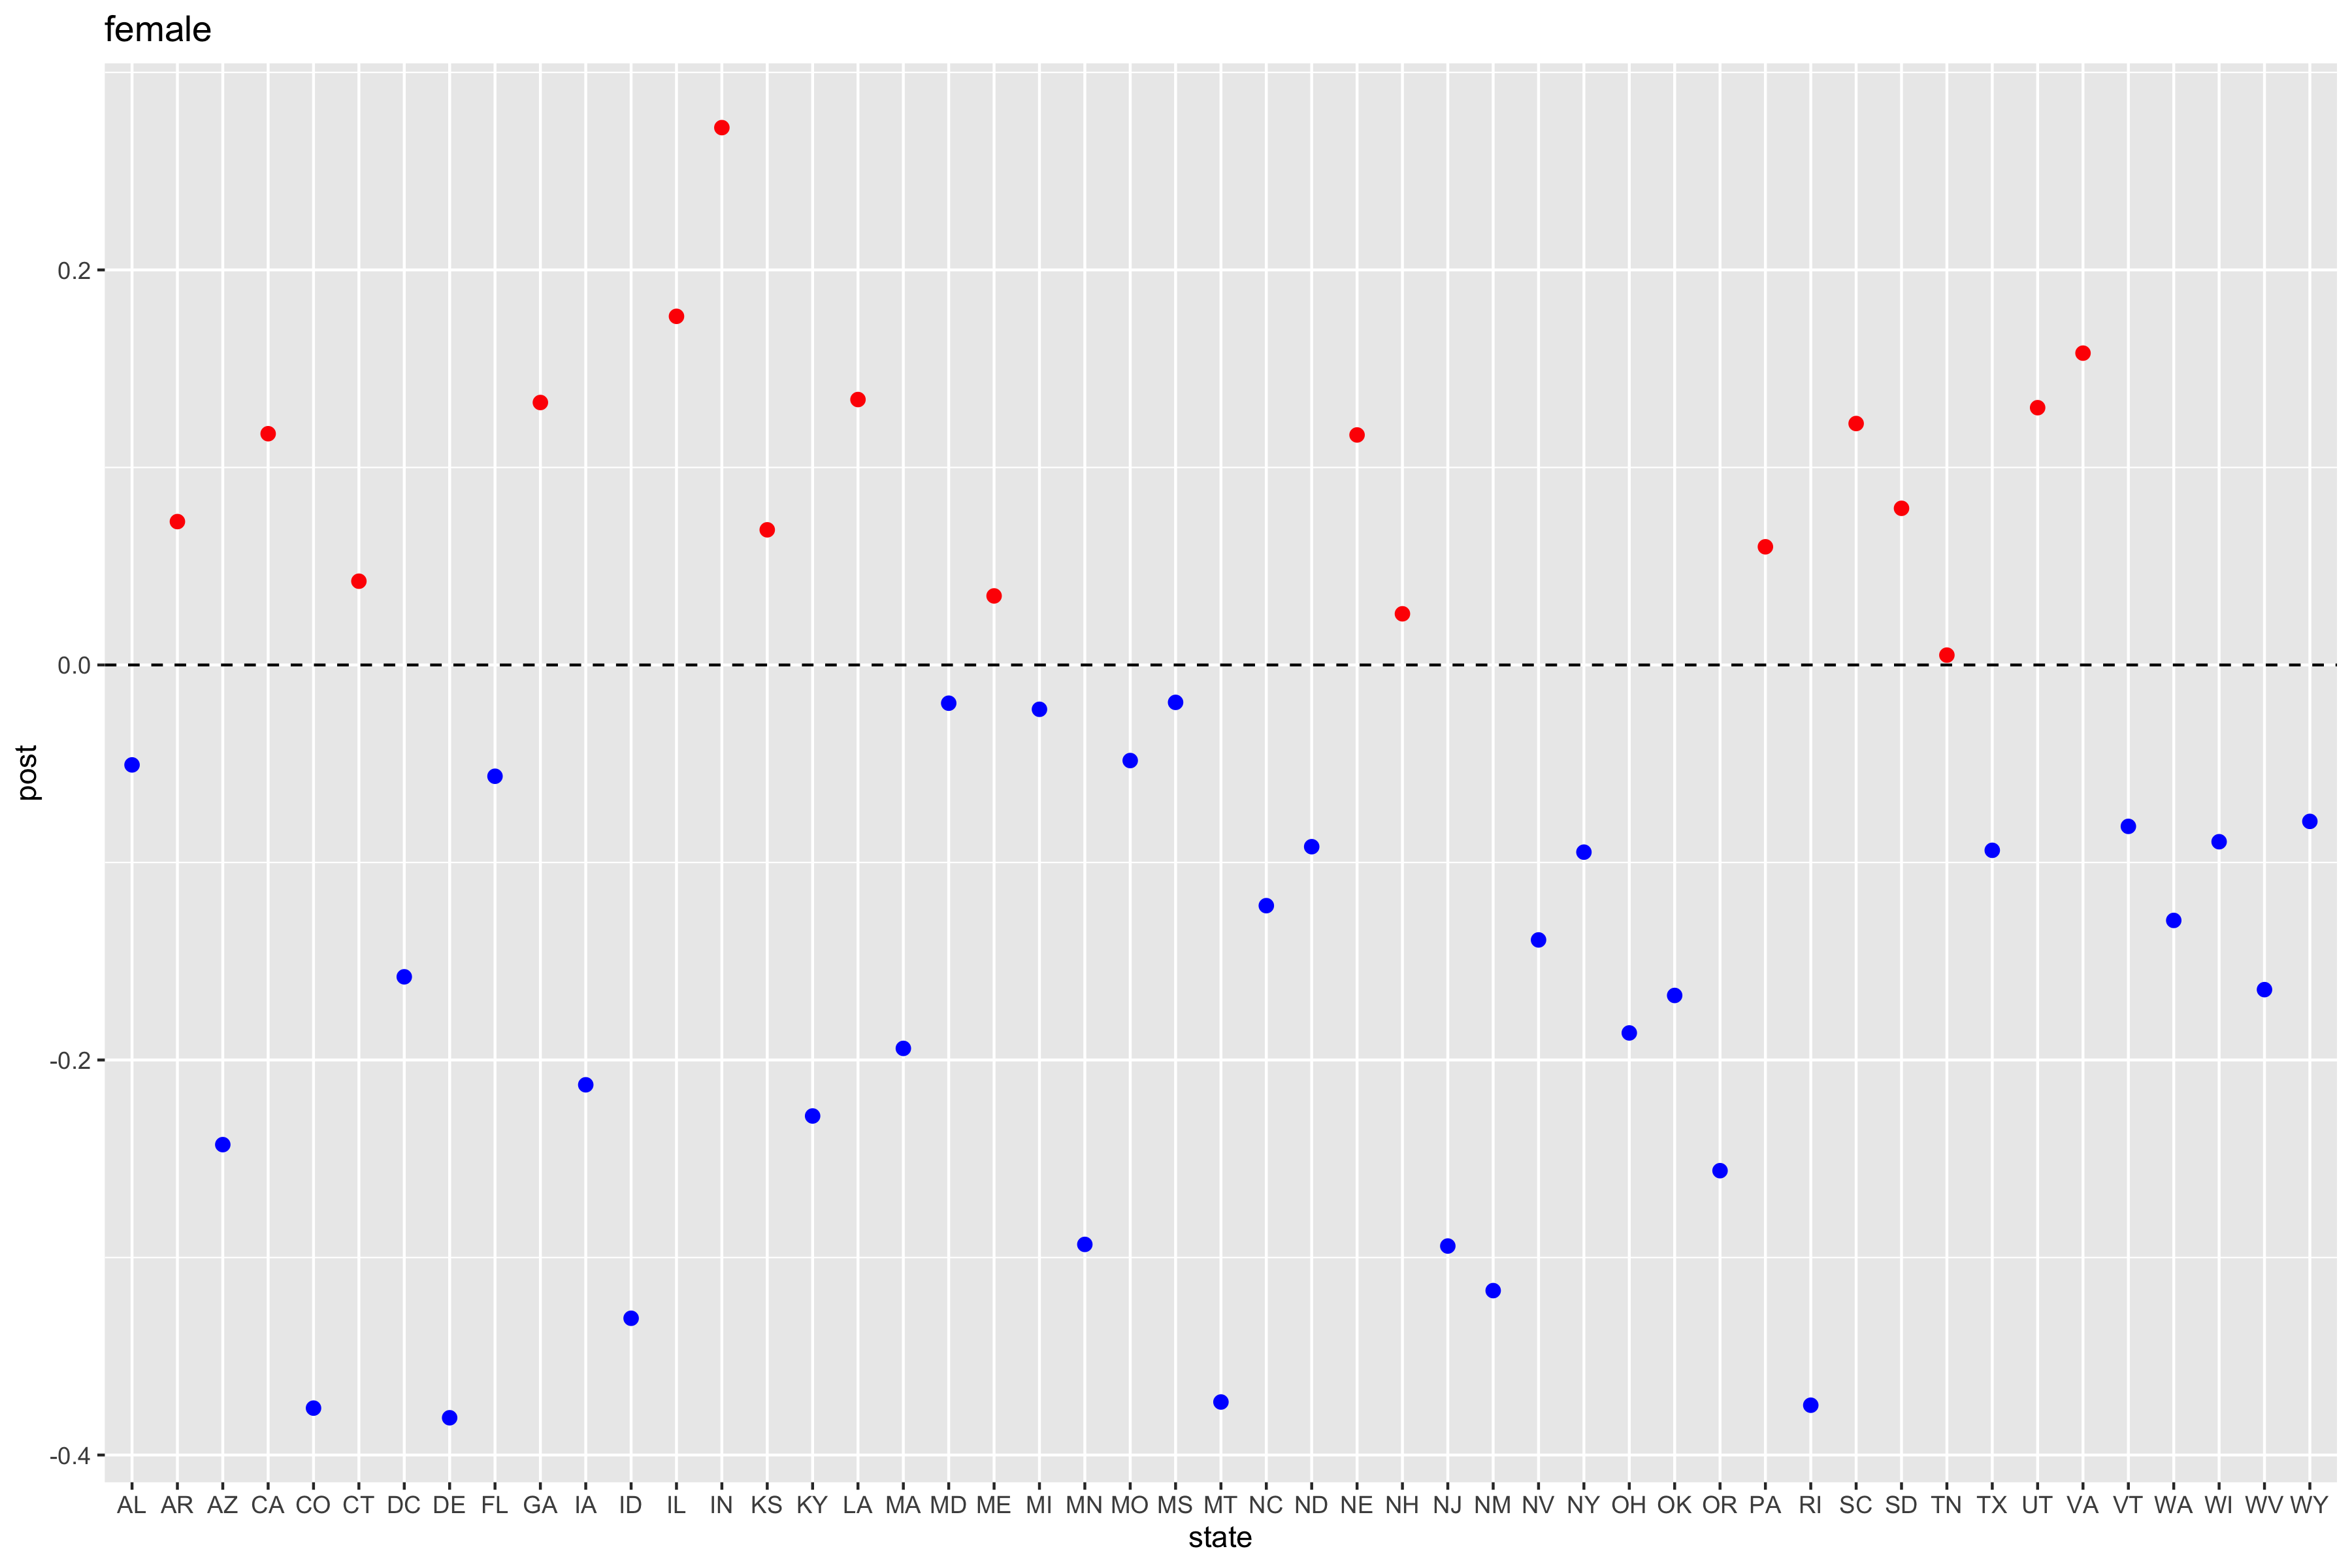
\includegraphics[width=\linewidth]{Ex5/figures/2post covariates8.png} 
        %\caption{Competitors} \label{fig:timing2}
    \end{subfigure}
    %\caption{Posterior estimates of the covariates.}
\end{figure}

\begin{figure}

    \centering
    \begin{subfigure}[t]{0.9\textwidth}
        \centering
        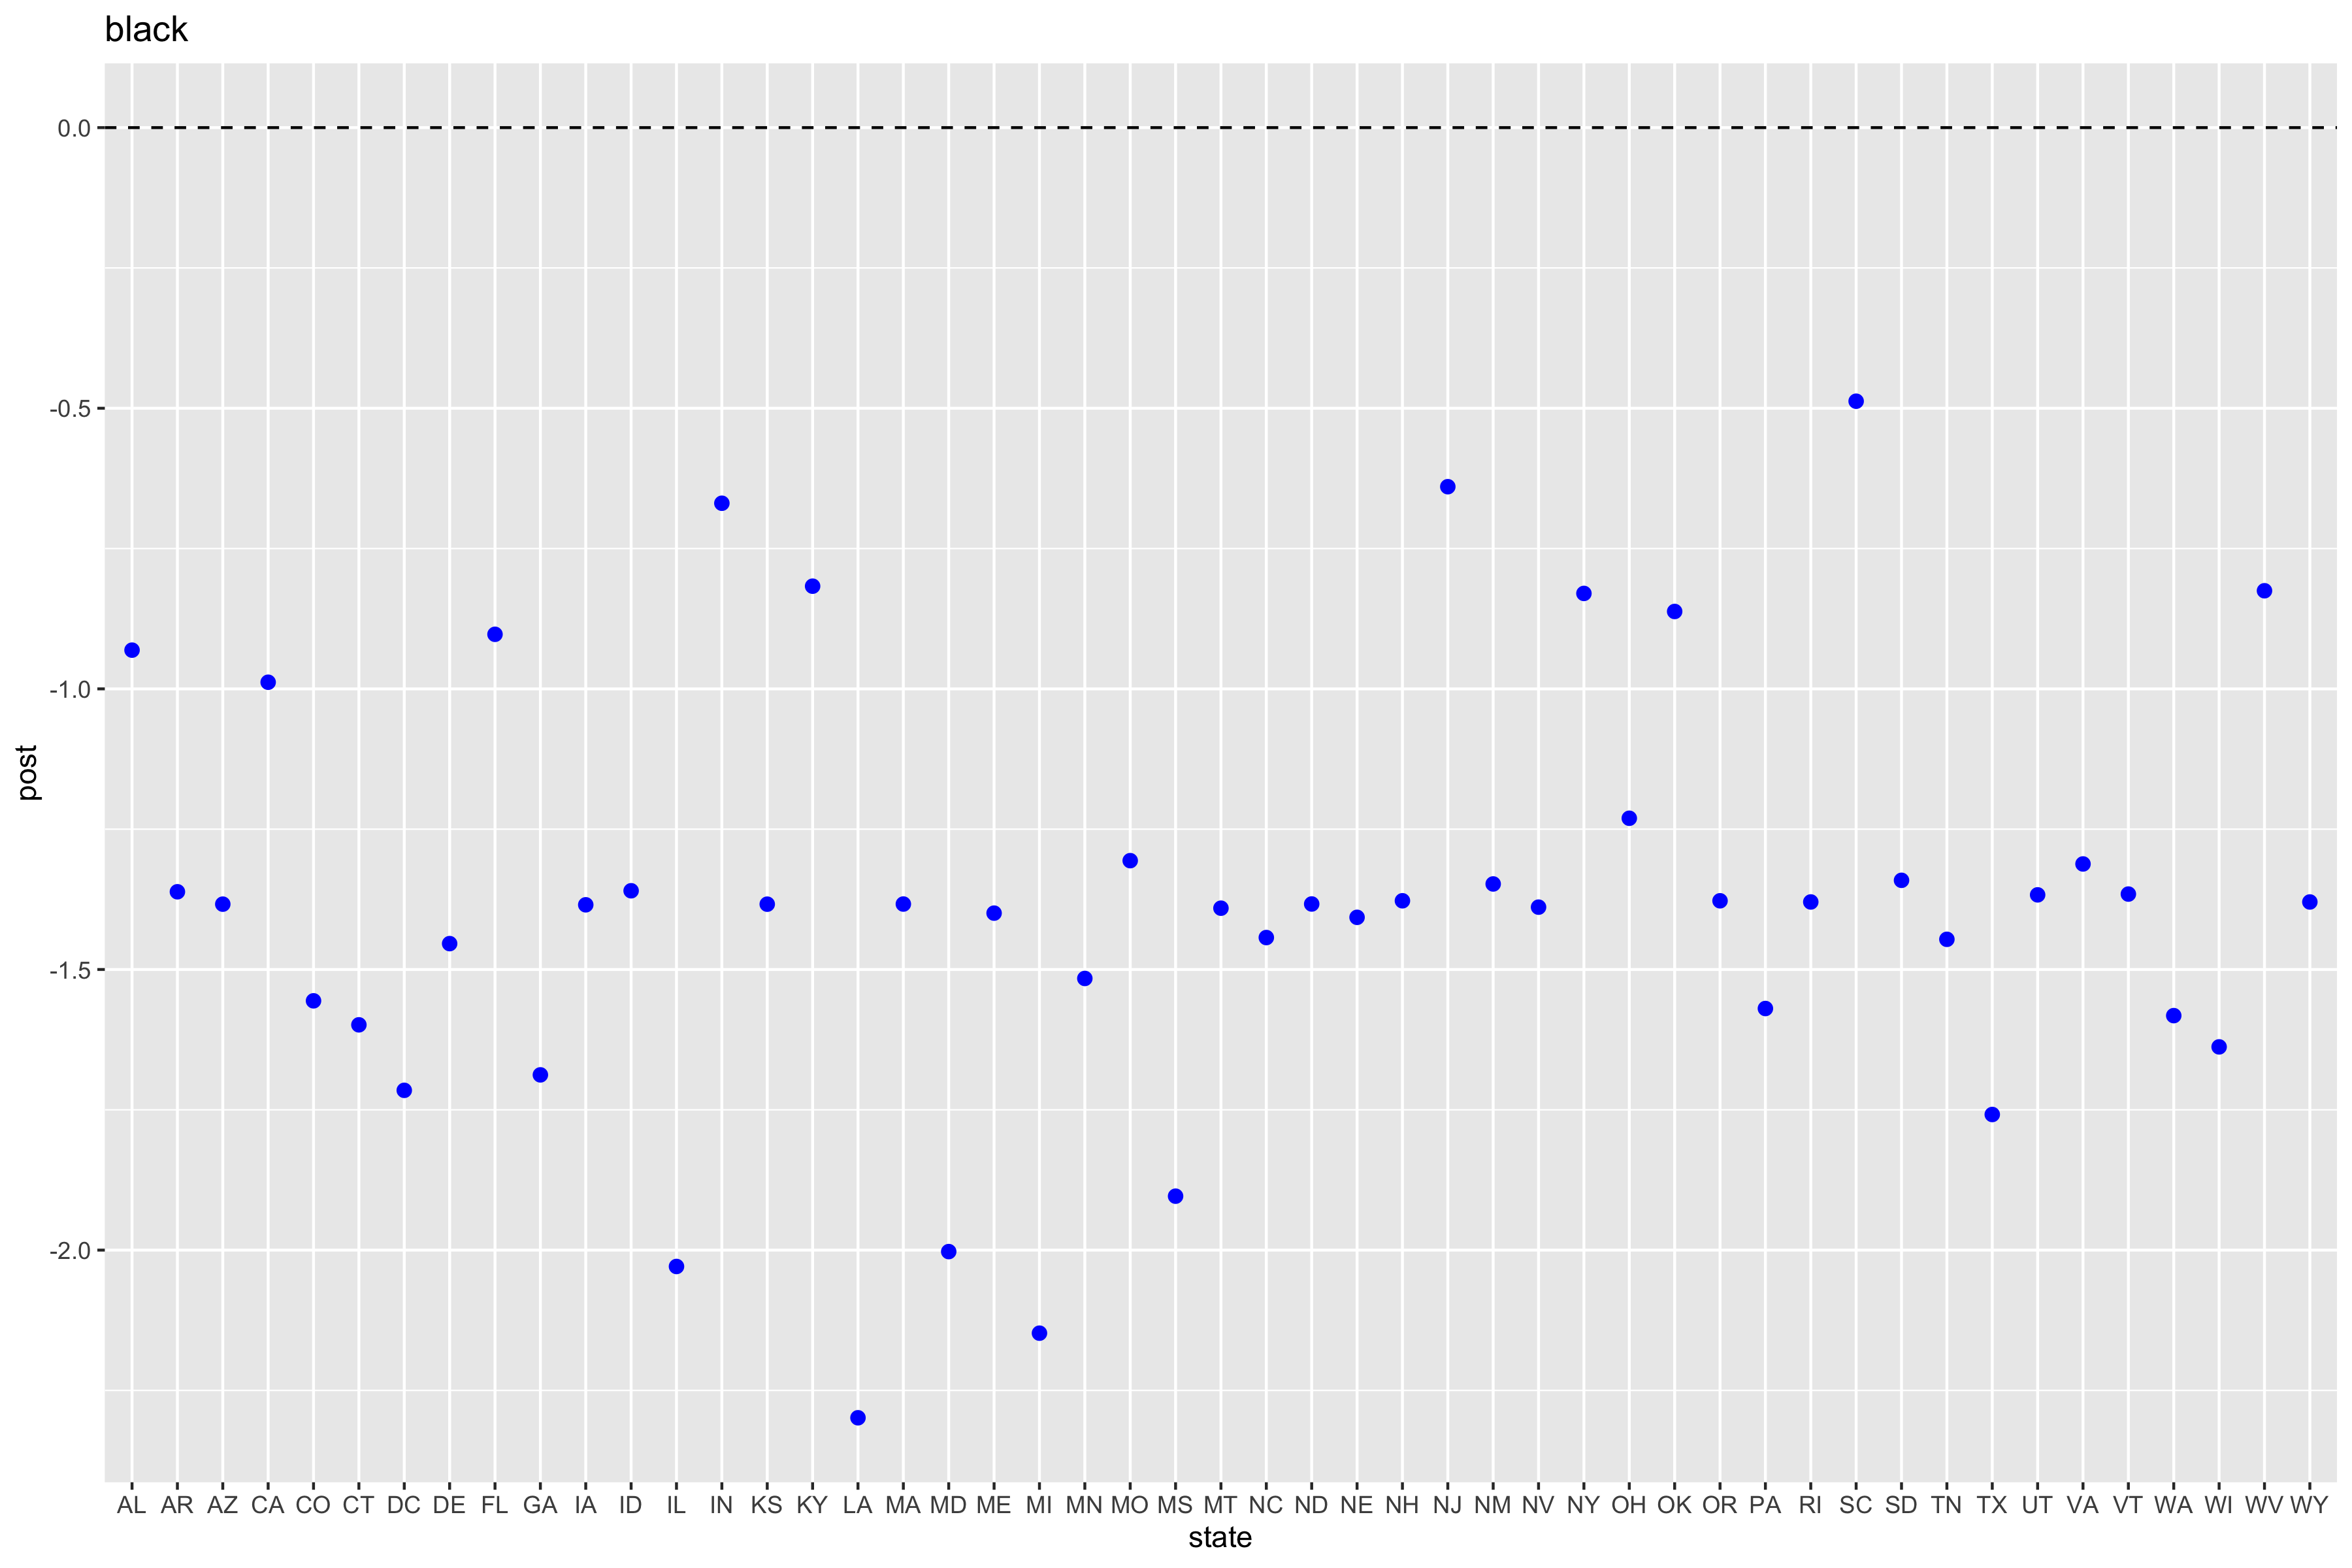
\includegraphics[width=\linewidth]{Ex5/figures/2post covariates9.png} 
        %\caption{Generic} \label{fig:timing1}
    \end{subfigure}
    \hfill
    \begin{subfigure}[t]{0.9\textwidth}
        \centering
        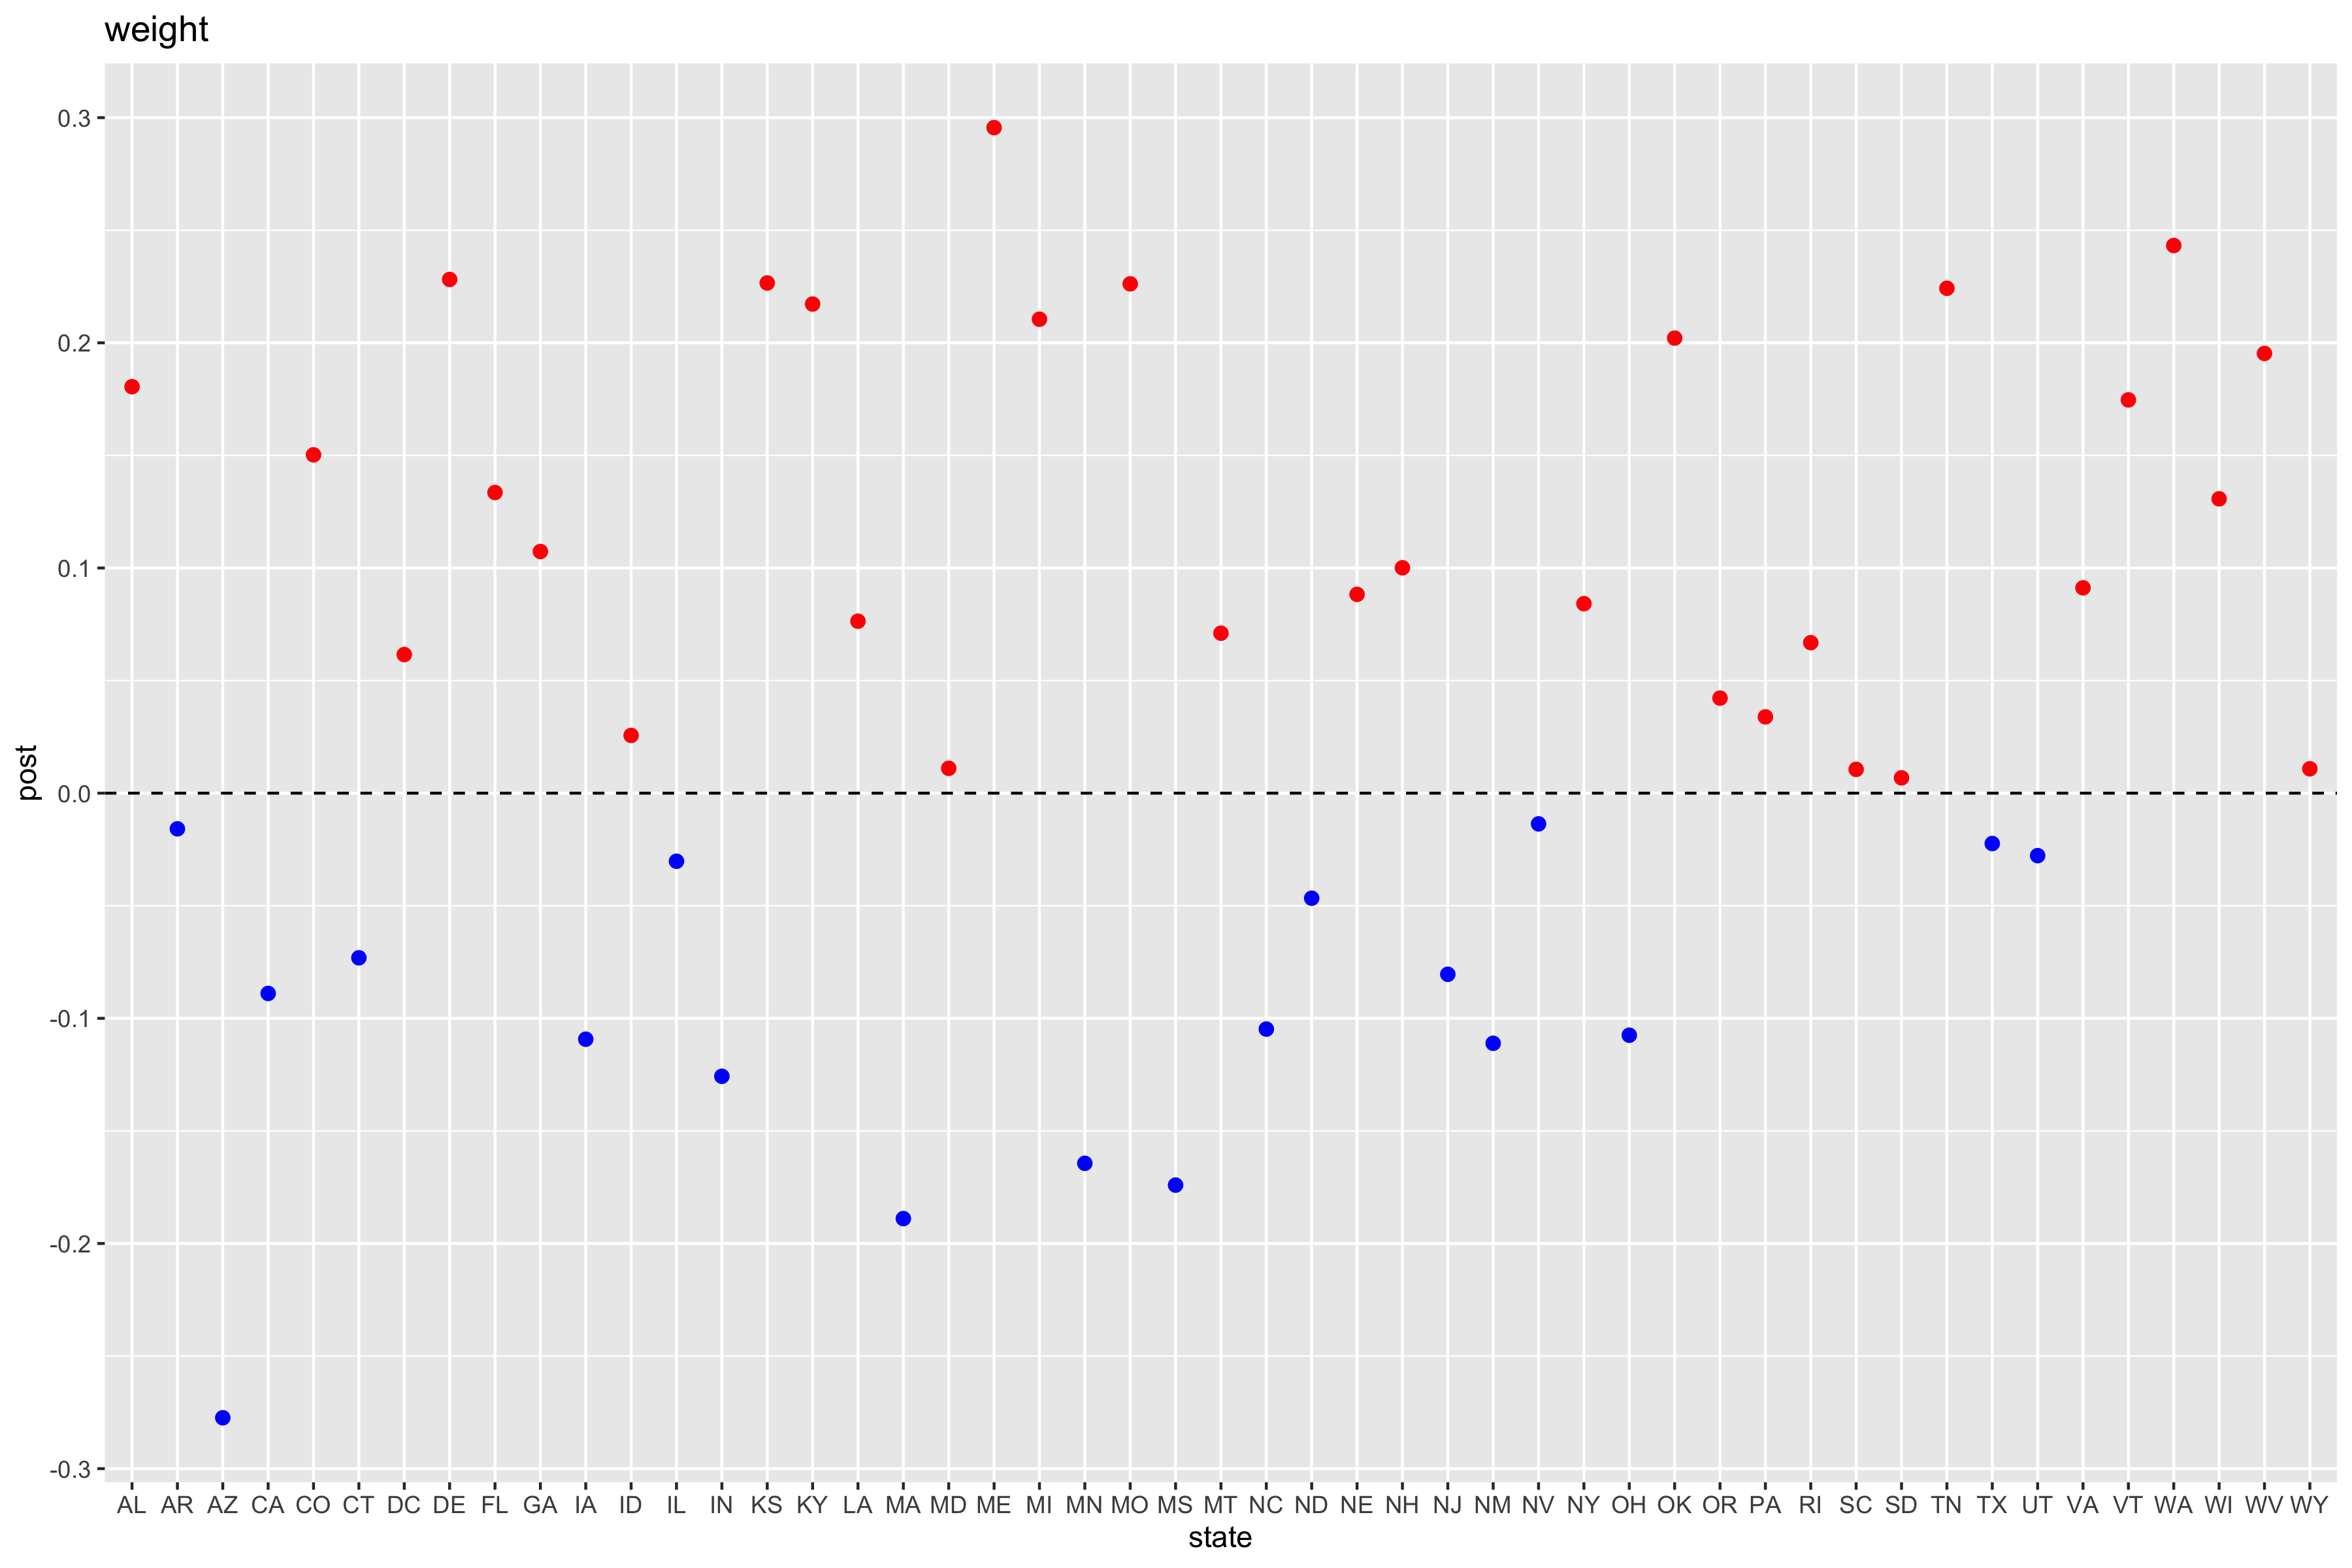
\includegraphics[width=\linewidth]{Ex5/figures/2post covariates10.png} 
        %\caption{Competitors} \label{fig:timing2}
    \end{subfigure}
    \caption{Posterior estimates of the covariates for each state.}
\end{figure}

\begin{figure}

    \begin{subfigure}[t]{0.9\textwidth}
        \centering
        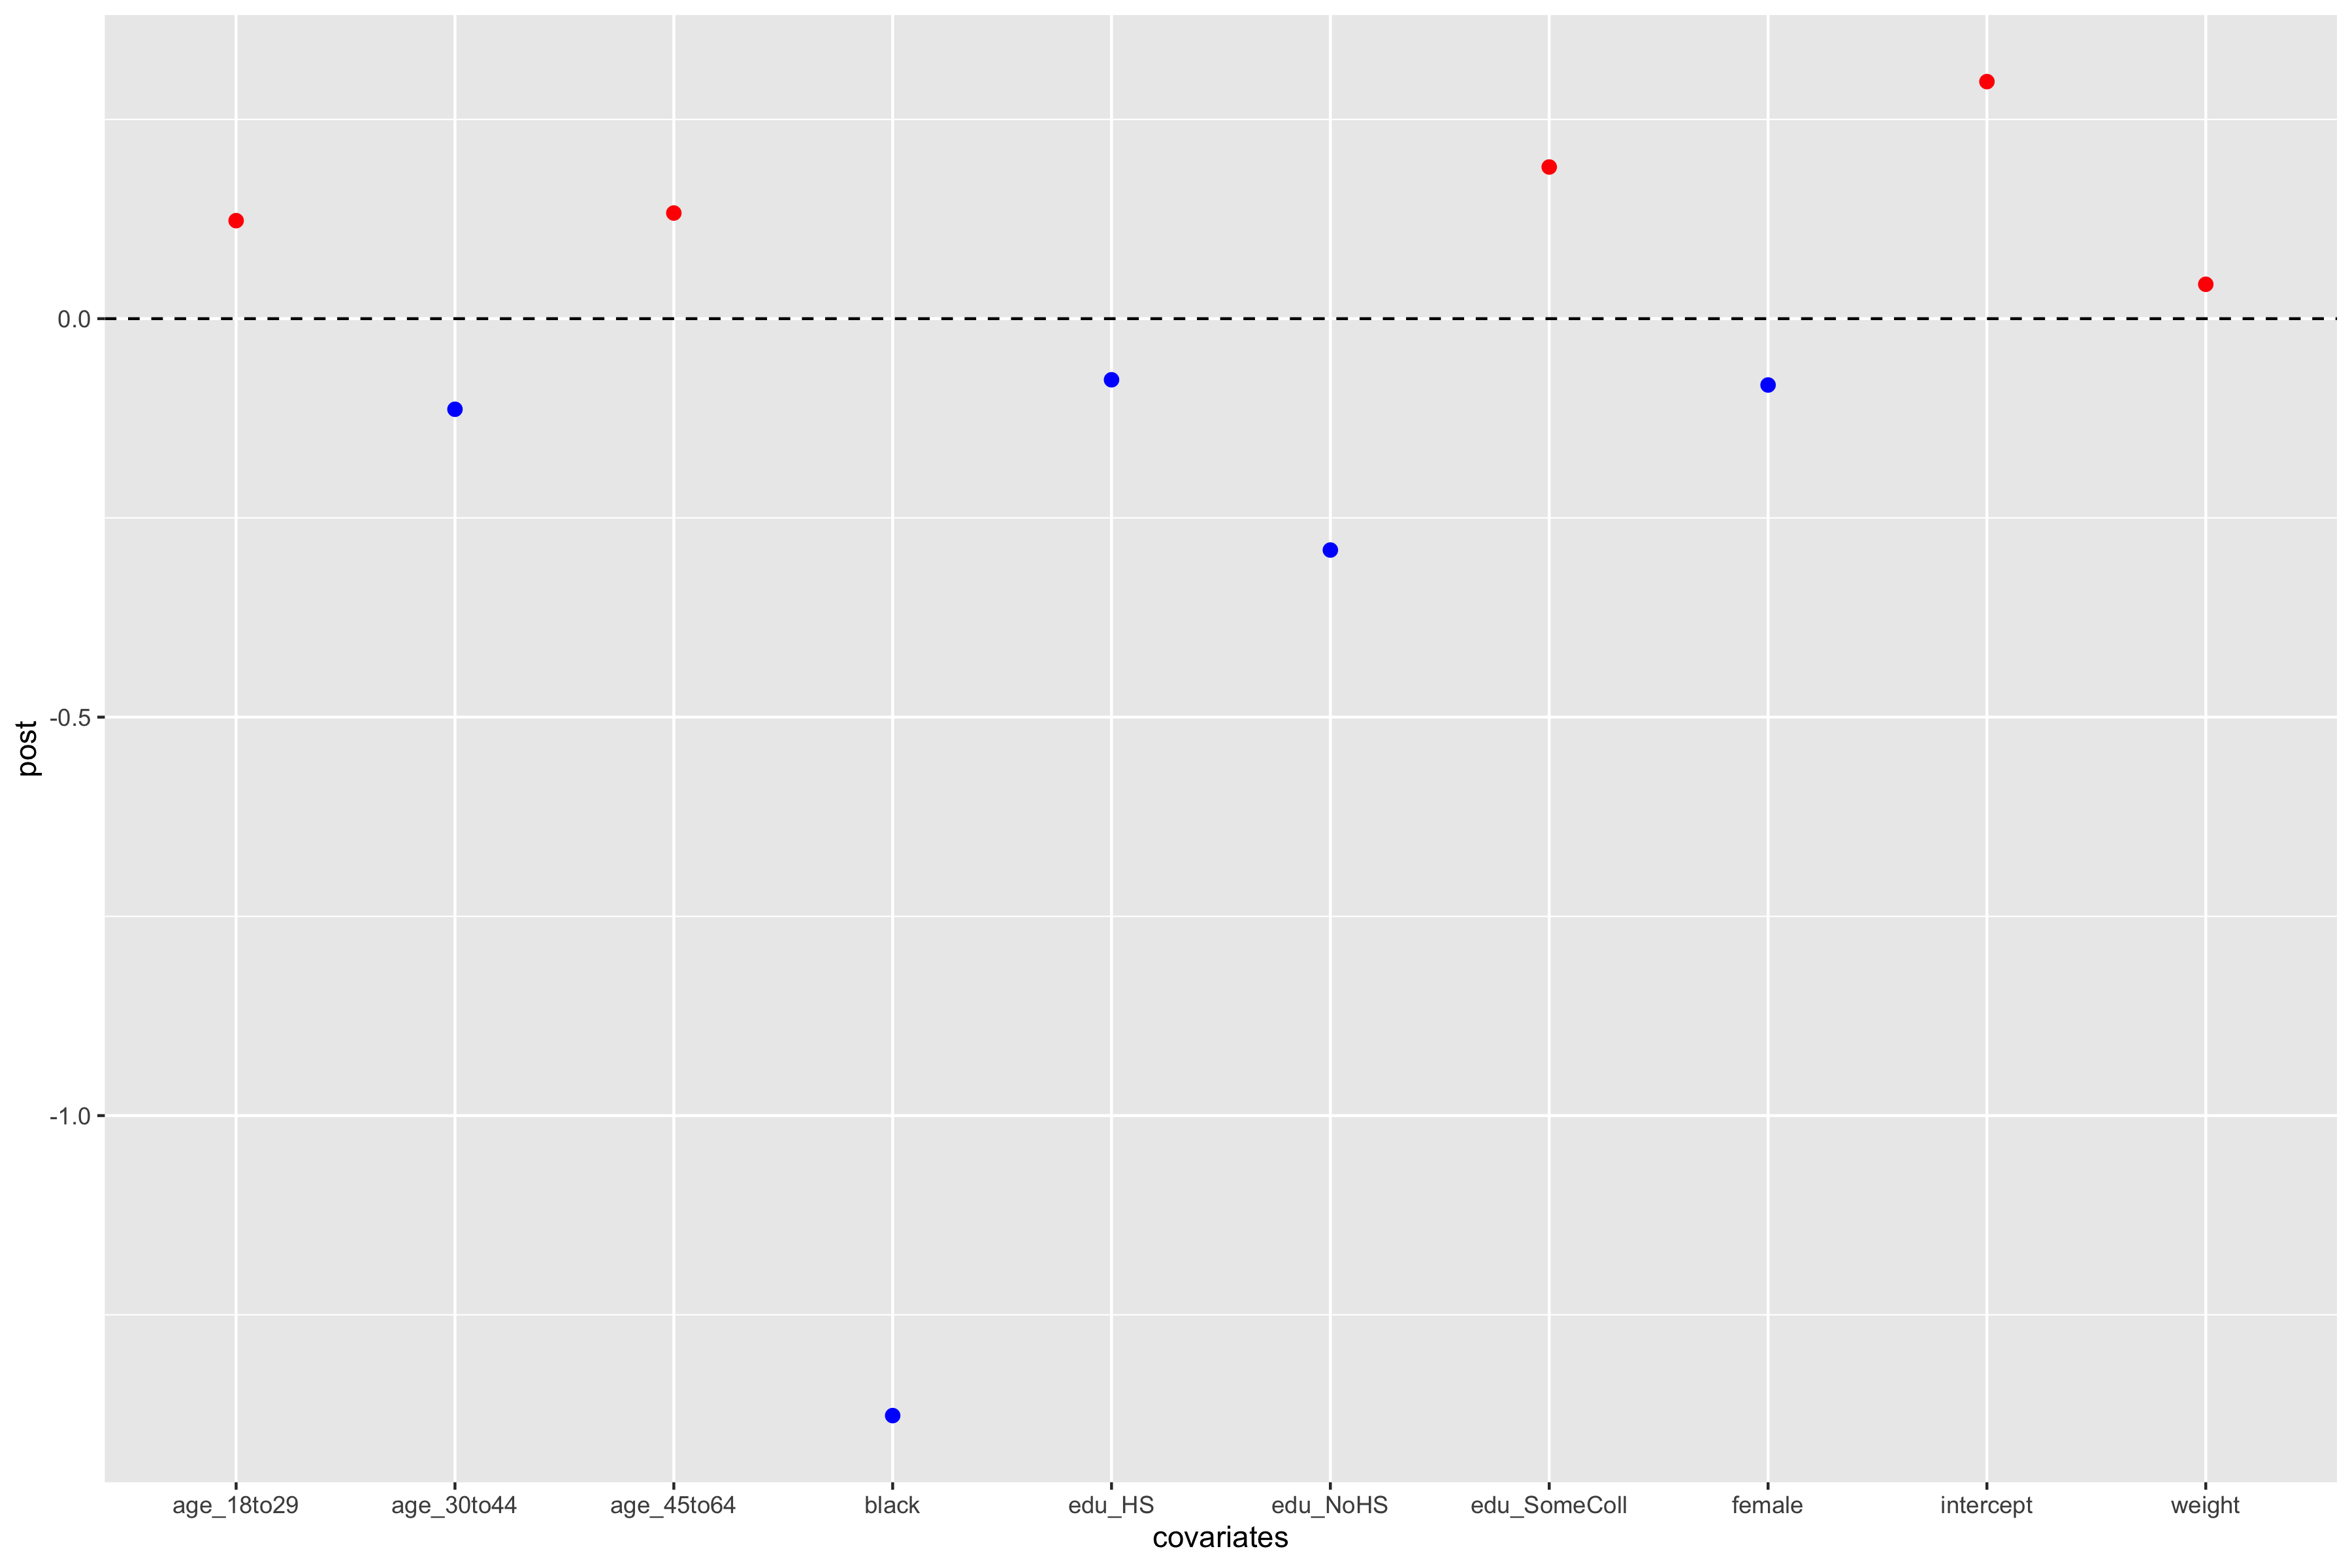
\includegraphics[width=\linewidth]{Ex5/figures/2post covariates0.png} 
        %\caption{Competitors} \label{fig:timing2}
    \end{subfigure}
    \caption{Posterior estimates of the covariates.}
\end{figure}

\end{document}

